\documentclass[../document.tex]{subfiles}
\begin{document}
\chapter{Results}
\label{chap: results}
In this section, we evaluate five convolutional neural networks: the model proposed by Chavez-Garcia et all \cite{omar2018traversability} and the four MicroResnet presented in the last chapter. We will select the best performing one based on the classification score on the test set. We will show the results of the same architecture trained on regression instead of classification and prove the latter yields better results. Finally, we qualitatively evaluate the best model by predicting traversability in real-world terrains. 
\section{Hardware}
% \subsection{Hardware}
We run all the experiment on a Ubuntu 18.10  work station equipped with a Ryzen 2700x, a powerful CPU with 8 cores and 16 threads, and a NVIDIA 1080 GPU with 8GB of dedicated RAM.
% \subsection{Dataset}
% To perform classification, we selected a threshold of twenty centimeters, according to the process explained in section \ref{sec: label-patches}, on a time window  of two seconds to label the patches, meaning that a patch with an advancement less than $20$ centimeters are labeled as \emph{no traversable} and vice-versa. For the regression thanks, we did not label the patch and directly regress on the raw advancement.

\section{Experimental validation}
We selected as \emph{validation} set ten percent of the training data. Since we stored each run of Krock as a \emph{.csv} file, validation and train set do not overlap.

% We also assessed the model's performance on the \emph{arck rocks} map, a $10\times10$m terrain with a big rocky bump in the middle.
% The test set is composed entirely by the quarry map \ref{fig : real-maps-quarry}, a real-world terrain. Table \ref{table: maps} describes in detail the configuration used in to generate all datasets.

\subsection{Metrics}
\paragraph{Classification:} To evaluate the model's classification performance we used two metrics: \emph{accuracy} and \emph{AUC-ROC Curve}. Accuracy scores the number of correct predictions made by the network while the AUC-ROC Curve represents degree or measure of separability, informally it tells how much model is capable of distinguishing between classes. For each experiment, we selected the model with the higher AUC-ROC Curve during training to be evaluated on the test set.

\paragraph{Regression:} We used the Mean Square Error to evaluate the model's performance.

\section{Training setup}
Initially, to train the models we first used Standard Gradient Descent with momentum set to $0.95$, weight decay to $1e-4$ and an initial learning rate of $1e-3$ as was originally proposed in He et al. \cite{he2015deep}. However, we later switched Leslie Smith's 1cycle policy \cite{1cycle} that allowed us to train the network faster and with higher accuracy. The average training time is $\approx 10$ minutes. We minimized the Binary Cross Entropy (BCE) for the classifier and the  Mean Square Error (MSE) for the regressor.

\section{Quantitative results}
\subsection{Model selection}
We compared the four different MicroRenset architectures \ref{subsec : micro-resnet} and the Vanilla CNN \ref{subsec : vanilla-cnn} proposed in the original work \cite{omar2018traversability} on the test set using as metric the ROC AUC.  Ideally, the second MicroResnet model should be able to extrapolate more features from the patch thanks to the big kernel size. We evaluated those models using a time window of two seconds, a threshold of $20$cm and we applied data augmentation as we described in section \ref{sec: data-aug}. We run five experiments per architecture and we selected the best performing network. Table \ref{tab : models-results-comparison} shows the results for each architecture. The best performing model was MicroResNet7x7-SE that obtained a ROC AUC of 0.896 on the test set. Moreover, the Squeeze and Excitation operator improved the performance of both MicroResNet3x3 and MicroResNet7x7 but only latter gained a huge boost of $0.021$.
\begin{table*}[ht]
  \centering
  \ra{1.2}
  \begin{tabular}{@{}lcccc@{}}
    \toprule
    Model & \multicolumn{2}{c}{ROC AUC} & Params \\ 
    \cline{1-4}
    & Mean & Top &  \\ 
    \cline{1-4}
    Vanilla  & 0.892& 0.890 &  974,351 \\
    MicroResnet3x3 & 0.881 & 0.883 & 302,610 \\
    MicroResnet3x3-SE & 0.883 & 0.888 & 313,64\\
    MicroResnet7x7 & 0.867 & 0.875 &  303,250\\
    MicroResnet7x7-SE &0.888 & \textbf{0.896} & 314,28\\
    \bottomrule   
  \end{tabular}
  \caption{Comparison of the four MicroResnet architectures \ref{fig : microresnet} and the original convolutional neural network (Vanilla CNN) proposed in the original work \cite{omar2018traversability} on the test set using as metrics the ROC AUC. The best performing model is MicroResNet7x7-SE.}
  \label{tab : models-results-comparison}
\end{table*}
\section{Final results}
\subsection{Classification}
Table \ref{tab : classification-results} table shows in deep the score of the best network for each dataset. We obtained $95\%$ accuracy and $0.96$ AUC on the validation set and $88\%$ accuracy and $0.89$ AUC on the test set.
\begin{table*}[htbp]
    \centering
    \ra{1.2}
    \begin{tabular}{@{}llccccc@{}}
    \toprule
    % \multicolumn{8}{c}{Quantitative evaluation in simulation} \\
    \multicolumn{2}{c}{Dataset} && \multicolumn{2}{c}{MicroResNet} & Size(m) & Resolution(cm/px) \\
    \cmidrule{1-2} \cmidrule{4-5}
    Type     &  Name  & Samples & ACC  &  AUC    & & \\
    \toprule
      \multirow{3}{*}{Synthetic}  & Training   & 429312 & - & - & $10\times10$ & 2\\
      &  Validation   & 44032 &  95.2 \% &  0.961 & $10\times10$ & 2 \\
      & Arc Rocks & 37273 &  85.5 \% &  0.888 & $10\times10$ & 2 \\
      \cmidrule{2-7}
    Real\\evaluation & Quarry & 36224 &  88.2 \%&  0.896& $32\times32$ & 2\\
    % \multirow{1}{*}{\makecell[l]{Real\\evaluation}} & Quarry & 36224 &  88.2 \%&  0.896& & 2\\
    \bottomrule   
\end{tabular}
\caption{Classification results on different datasets.}
\label{tab : classification-results}
\end{table*}

\subsection{Regression}
We regressed on the advancement using the best model selected previously, MicroResNet7x7-SE. Table \ref{tab : regression-results} table shows in deep the score of the best network for each dataset.
\begin{table*}[htbp]
    \centering
    \ra{1.2}
    \begin{tabular}{@{}llcccc@{}}
    \toprule
    % \multicolumn{8}{c}{Quantitative evaluation in simulation} \\
    \multicolumn{2}{c}{Dataset} & & \multicolumn{1}{c}{MicroResNet} & Size & Resolution(cm/px) \\
    \cmidrule{1-2} \cmidrule{4-5}
    Type     &  Name  & Samples & MSE      & \\
    \toprule
      \multirow{3}{*}{Synthetic}  & Training  &  - & - &$10\times10$  & 2\\
      &  Validation   & 44032 &  0.006  &  $10\times10$ & 2 \\
      & Arc Rocks & 37273 & 0.020  &  $10\times10$& 2 \\
      \cmidrule{2-6}
    Real\\evaluation & Quarry & 36224 &  0.022 & $32\times32$ & 2\\
    % \multirow{1}{*}{\makecell[l]{Real\\evaluation}} & Quarry & 36224 &  88.2 \%&  0.896& & 2\\
    \bottomrule   
\end{tabular}
\caption{Classification results on different datasets.}
\label{tab : regression-results}
\end{table*}
The regressor can be used to classify patches using different thresold by just see if the predicted advancement is greater or lower than a threshold. However, we always need to fix a threshold to estimate traversabilit. Once the value is fixed, the same model trained on the same dataset to classify patches drastically outperforms the regressor. Table \ref{tab : reg-clas} shows the accuracy of two MicroResNet7x7-SE on classification and regression after a threshold of twenty centimeters is selected. For this reason, we choose the MicroResNet7x7-SE trained on the classification task to be evaluated.
\begin{table*}[htbp]
  \centering
  \ra{1.2}
  \begin{tabular}{@{}lcc@{}}
  \toprule
  &  Regression & Classification  \\
 & \multicolumn{2}{c}{ACC} \\ 
  \cline{2-3}
   Top & $72.8\%$ & \textbf{88.2\%} \\
   Mean & $73.6\%$ & \textbf{87.8\%} \\
  \bottomrule   
\end{tabular}
\caption{Regression and classification accuracy for the same model,  MicroResNet7x7-SE, once a threshold of $20$cm is fixed. The classifier outperforms the regressor by $15\%$.}
\label{tab : reg-clas}
\end{table*}
% Moreover, we would like to also show the different steps we made to reach this result. The following table shows the metric's score without any data-augmentation.
% Adding dropout increases the results.
% With dropout plus coarse dropout.
\section{Qualitative results}
We qualitative evaluated the classifier predictions by plotting the traversability probability on different maps in 3D.  We used a sliding window to extract the patches from the tested maps to collect the model's predictions. Then, we created a texture based on the traversable probability, we have colored it using a colormap and finally applied on the 3D model of each map. We evaluated four rotations, from bottom to top, top to bottom, left to right and right to left since those are the most human understandable. By using those angles, we can optimize the cropping process since to avoid rotate each patch based on the Krock's head position. Instead, we can just rotate the entire map beforehand. 
\subsection{Quarry}
The first map we evaluate is Quarry, this map is $32\times 32$m long and has a maximum height of $10$m. We can use some of the terrain interesting features, such as are three bis slopes and the rocky ground on the top, to evaluate the model. For instance, w expect the trail on the slopes to be traversable at almost any rotation, especially from left to right and vice-versa. The top part should be hard to traverse in almost any case. Figure \ref{fig : quarry-trav} shows the traversability probability directly on the map. 
\todo[inline]{some where place the colormap bar}
\begin{figure} [htbp]
\centering
\begin{subfigure}[b]{0.45\textwidth}
  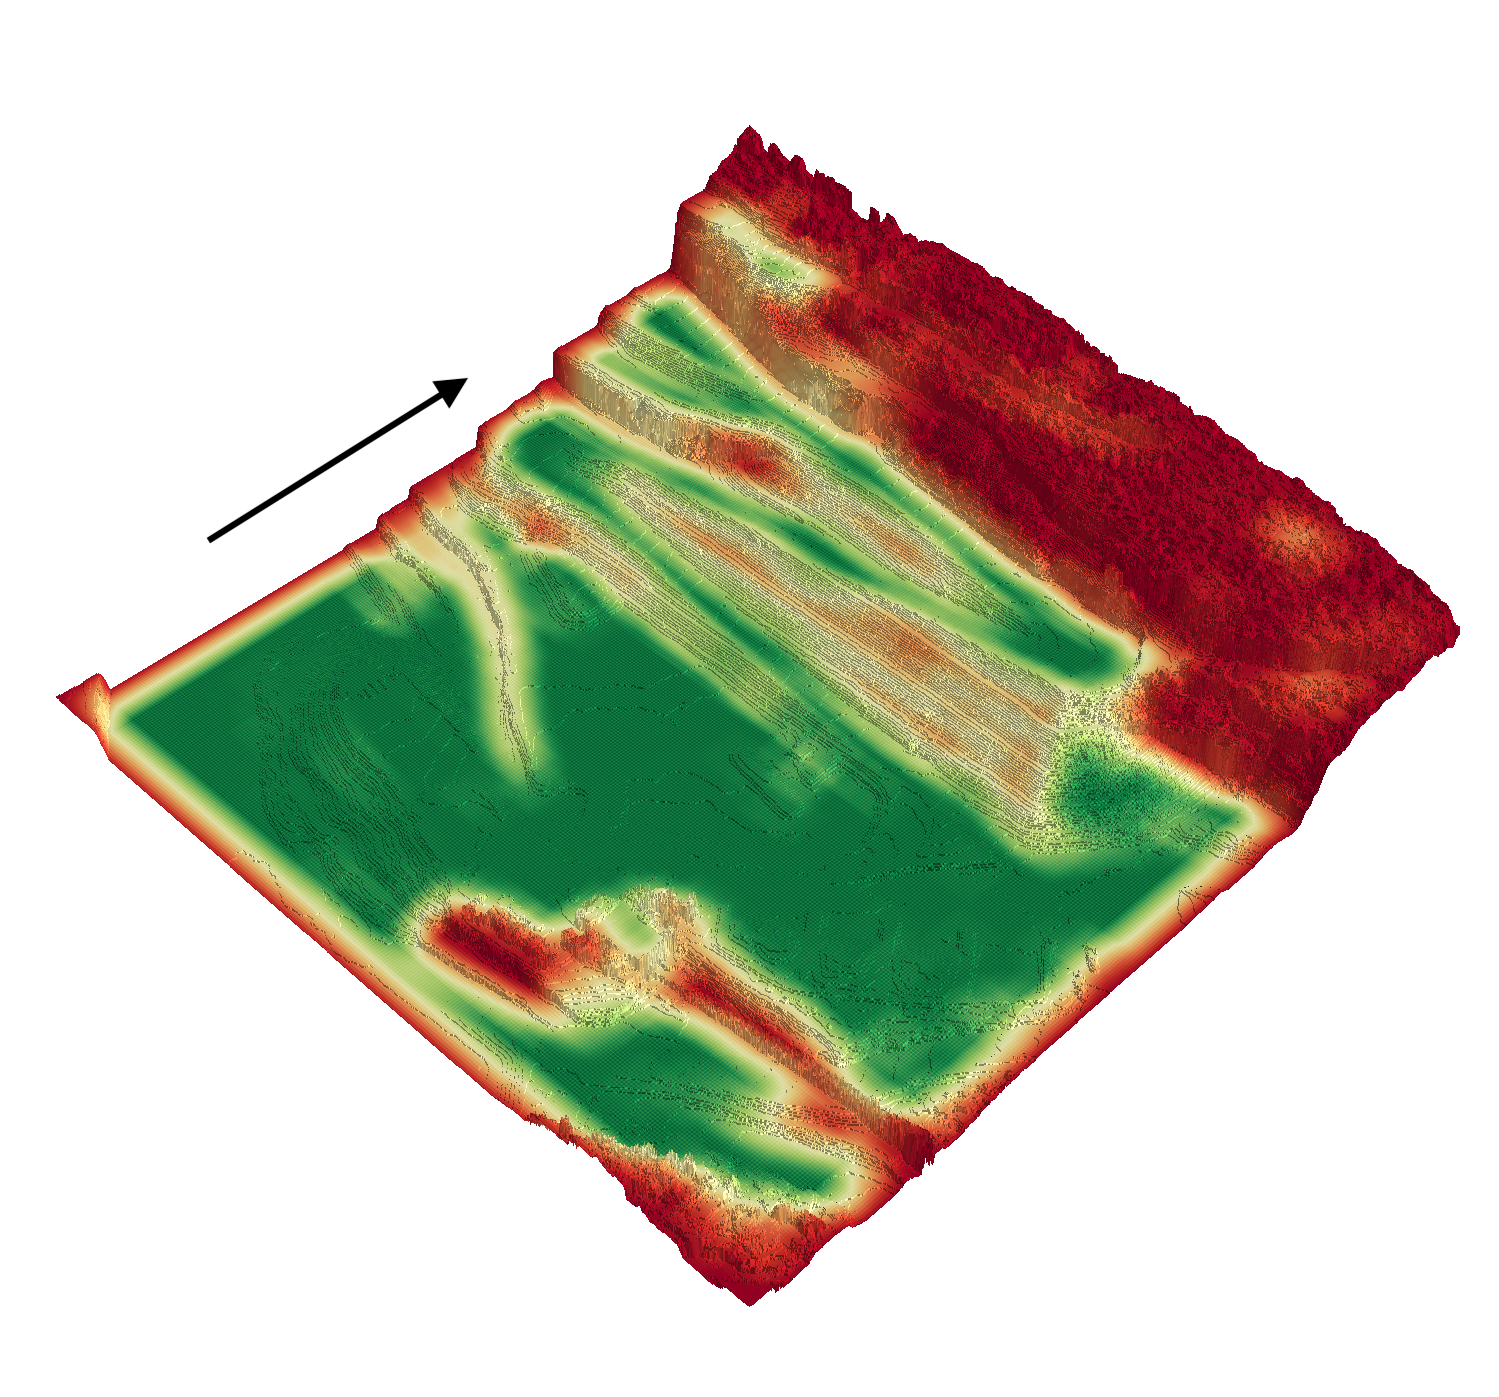
\includegraphics[width=\linewidth]{../img/4/traversability/quarry/-270.png} 
  \subcaption{Robot moving from bottom to top} 
  % \label{fig: quarry-b2t}
\end{subfigure}
\begin{subfigure}[b]{0.45\textwidth}
    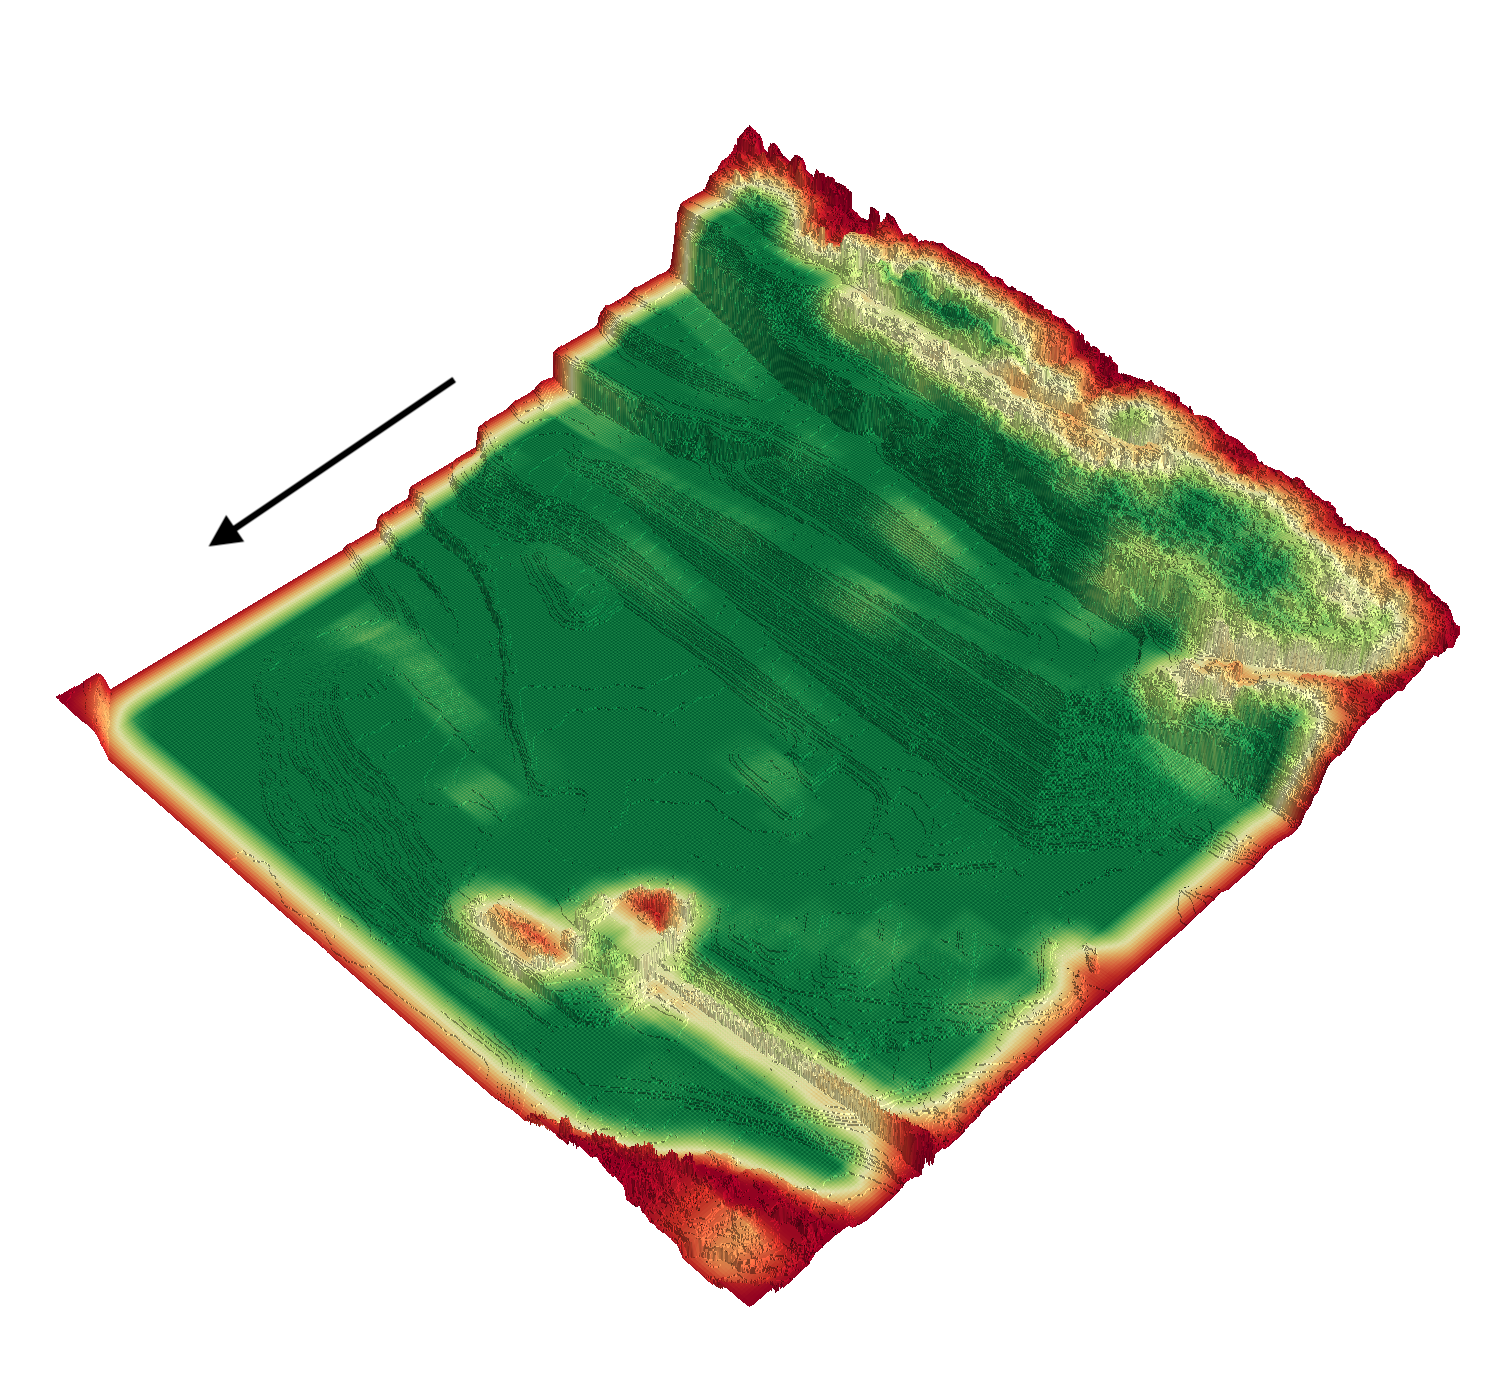
\includegraphics[width=\linewidth]{../img/4/traversability/quarry/-90.png}
    \subcaption{Robot moving from top to bottom} 
    % \label{fig: quarry-t2b}
\end{subfigure}
\begin{subfigure}[b]{0.45\textwidth}
  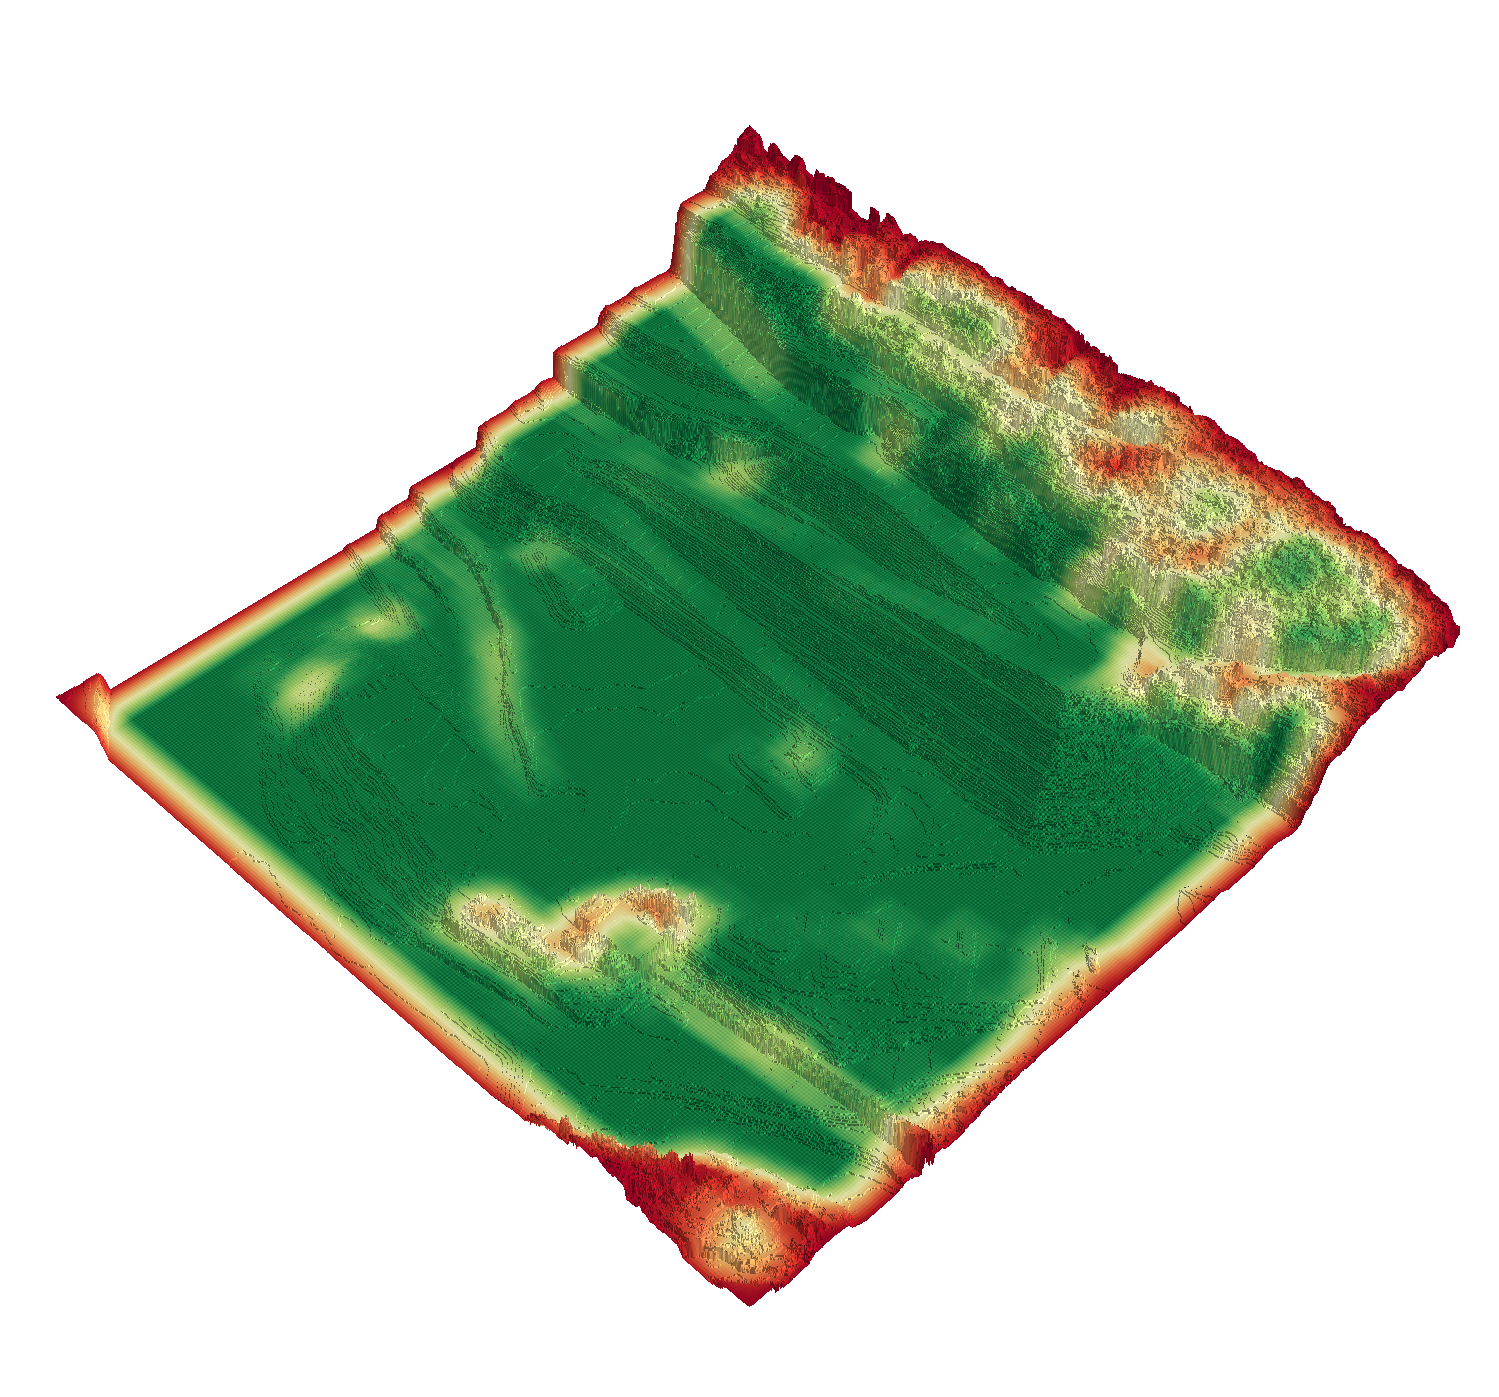
\includegraphics[width=\linewidth]{../img/4/traversability/quarry/-0.png}
  \subcaption{Robot moving from left to right}   
  % \label{fig: quarry-l2r}
\end{subfigure}
\begin{subfigure}[b]{0.45\textwidth}
    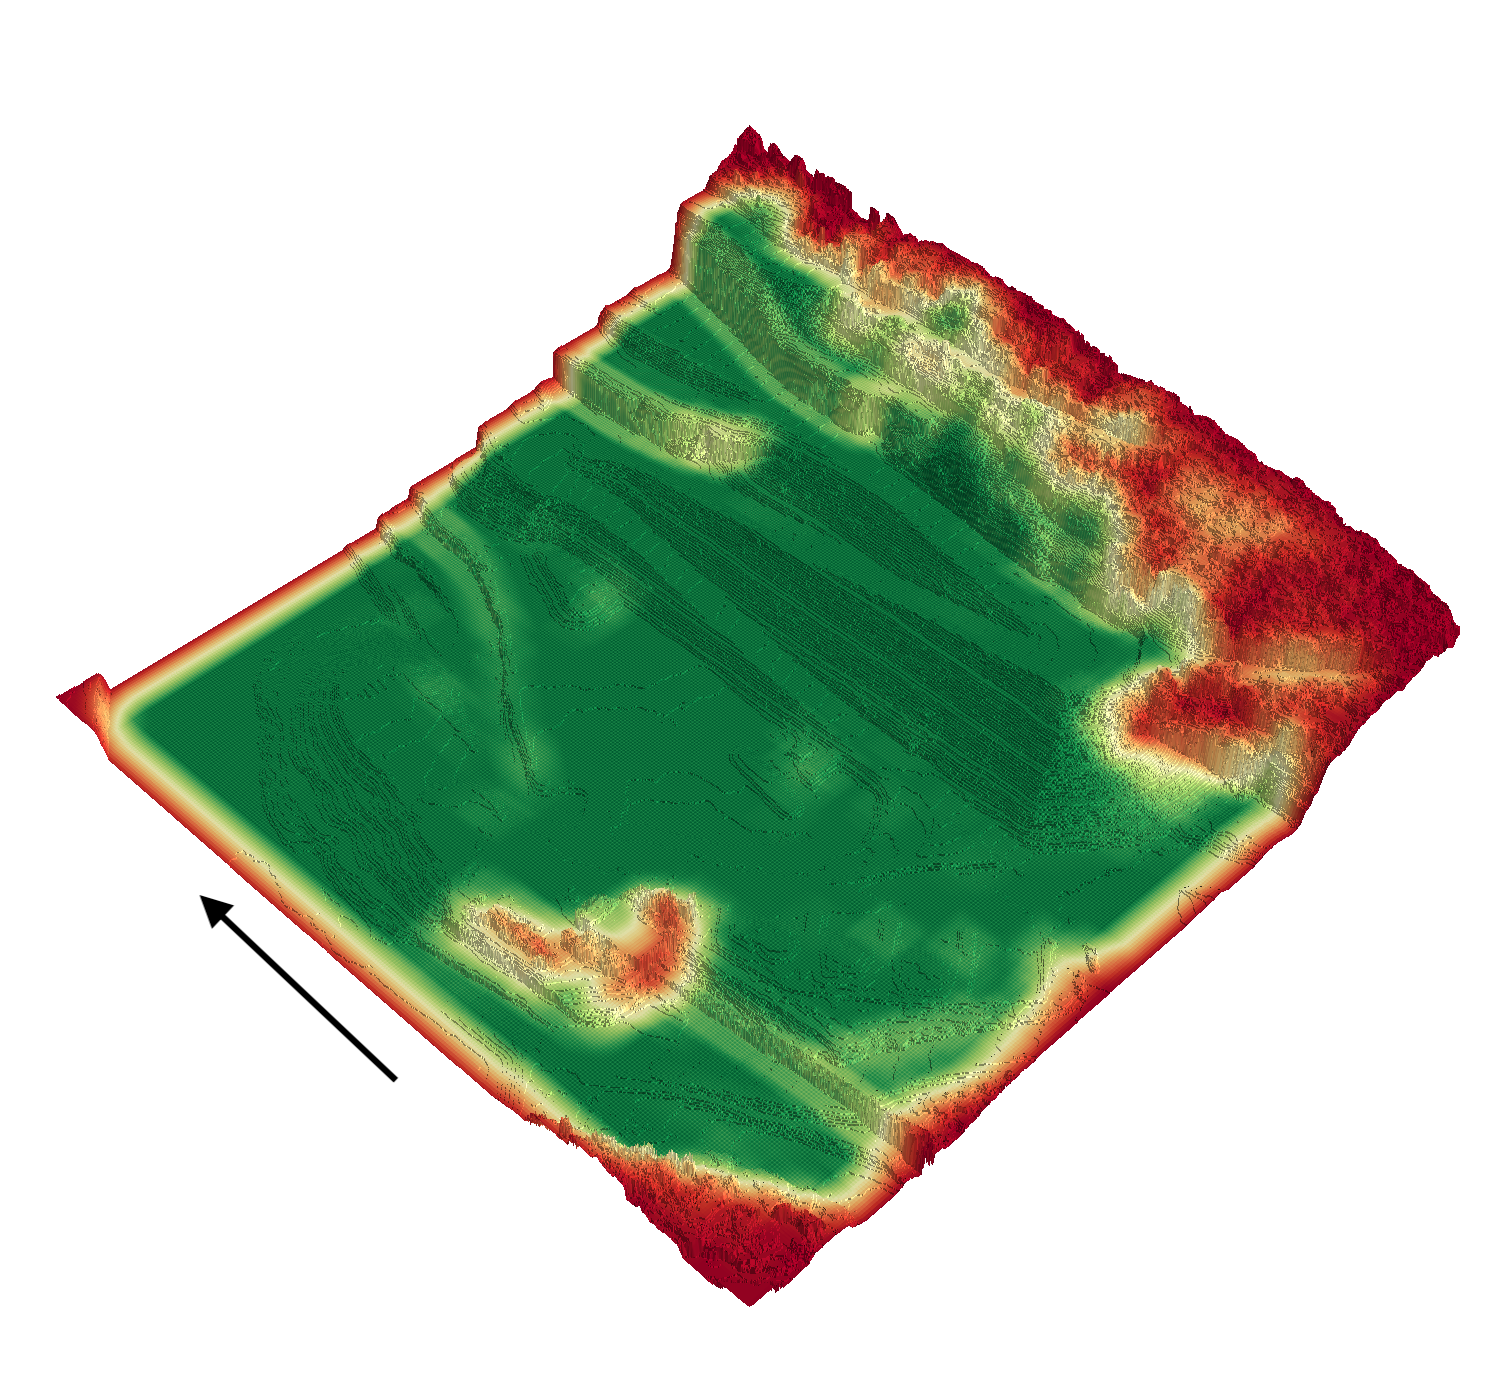
\includegraphics[width=\linewidth]{../img/4/traversability/quarry/-180.png}  
    \subcaption{Robot moving from right to left} 
    % \label{fig: quarry-r2l}
\end{subfigure}
\caption{Traversability probability on the Quarry map, $32\times 32$m, for different Krock's rotation. The values are obtained by sliding a window on the map to create the patches to predict their traversability.}
\label{fig : quarry-trav}
\end{figure}
 Correctly, the lower part of the map, composed by flat regions, was labeled with high confidence as traversable in all rotations. On the other hand, the traversability of the slopes and the bumps on the top region depends on the robot orientation.

\subsection{Bars}
Bars is a map composed of different heights wall, thus we expected similar probabilities with different orientation. Figure \ref{bars-trav} shows the traversability probabilities on the terrain.

\begin{figure} [htbp]
  \centering
  \begin{subfigure}[b]{0.45\textwidth}
    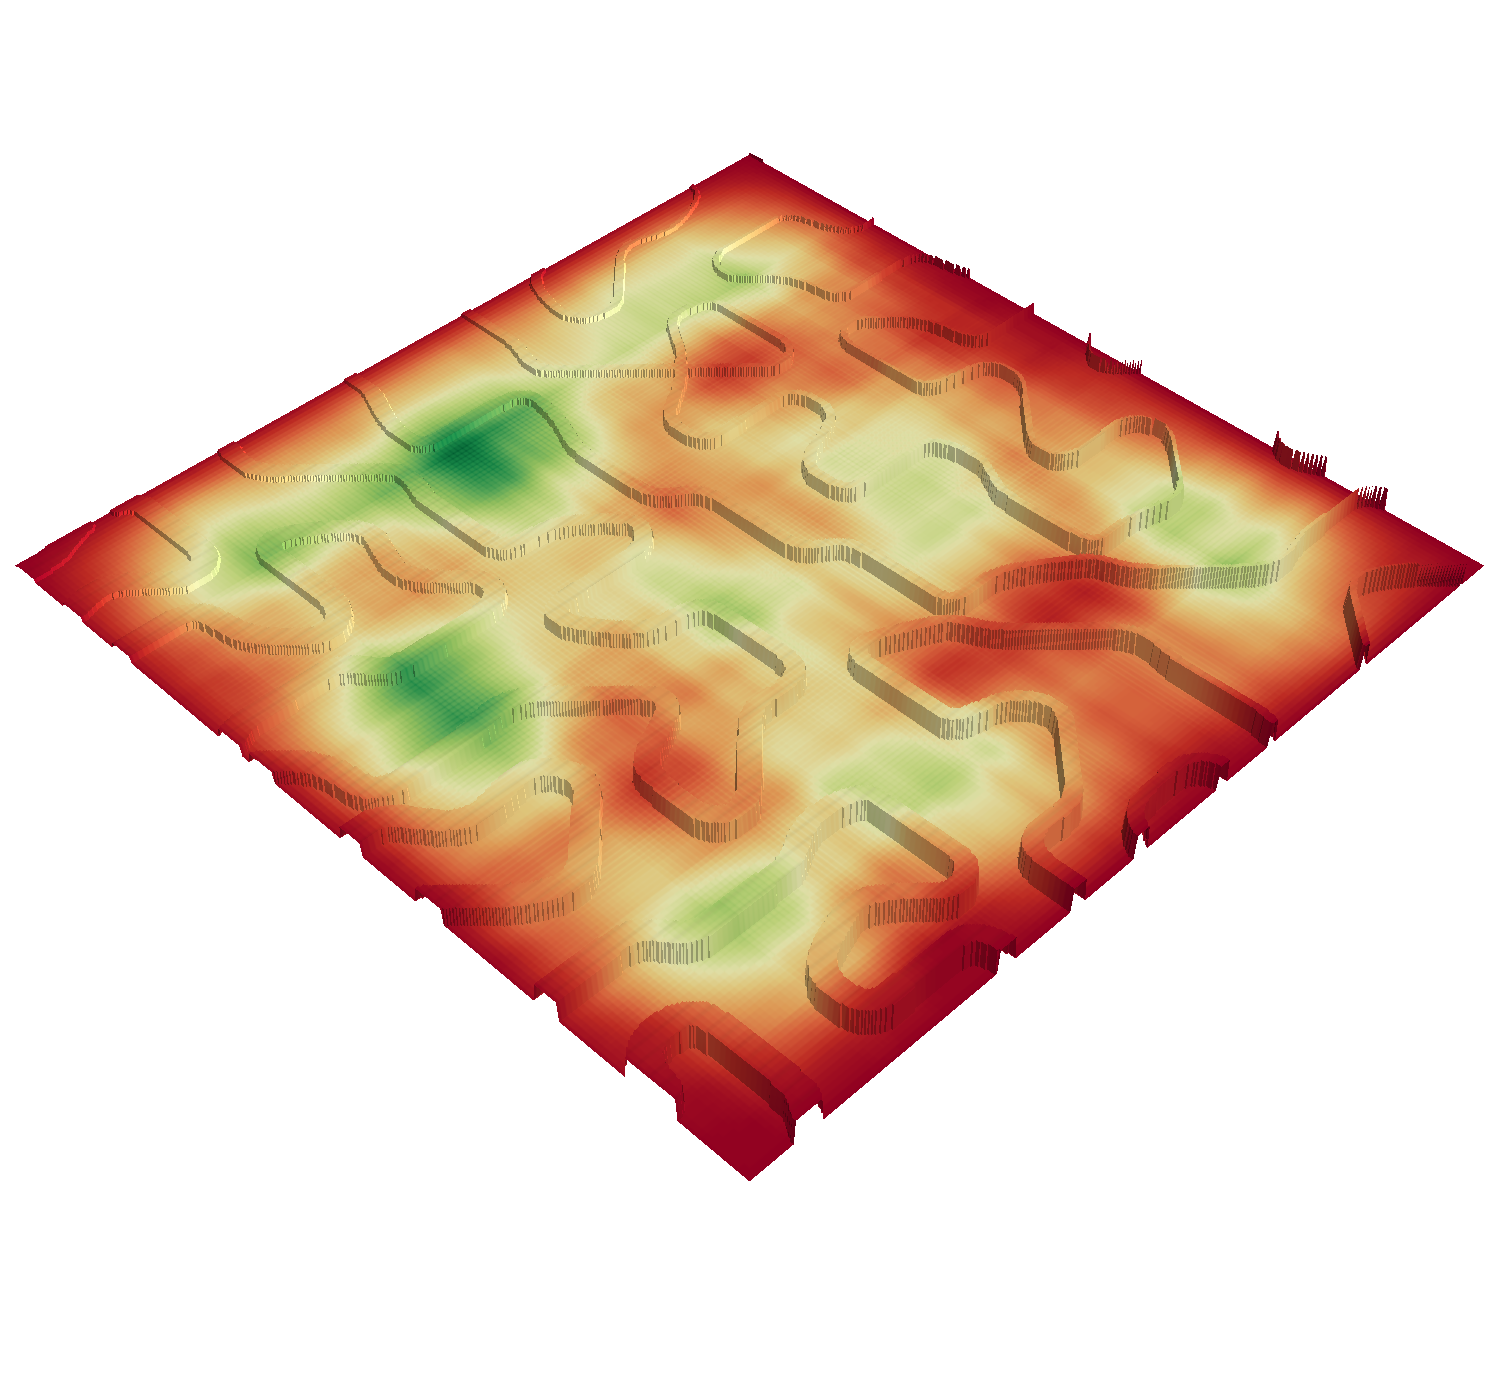
\includegraphics[width=\linewidth]{../img/4/traversability/bars/-270.png} 
    \subcaption{Robot moving from bottom to top} 
    % \label{fig: bars-b2t}
  \end{subfigure}
  \begin{subfigure}[b]{0.45\textwidth}
      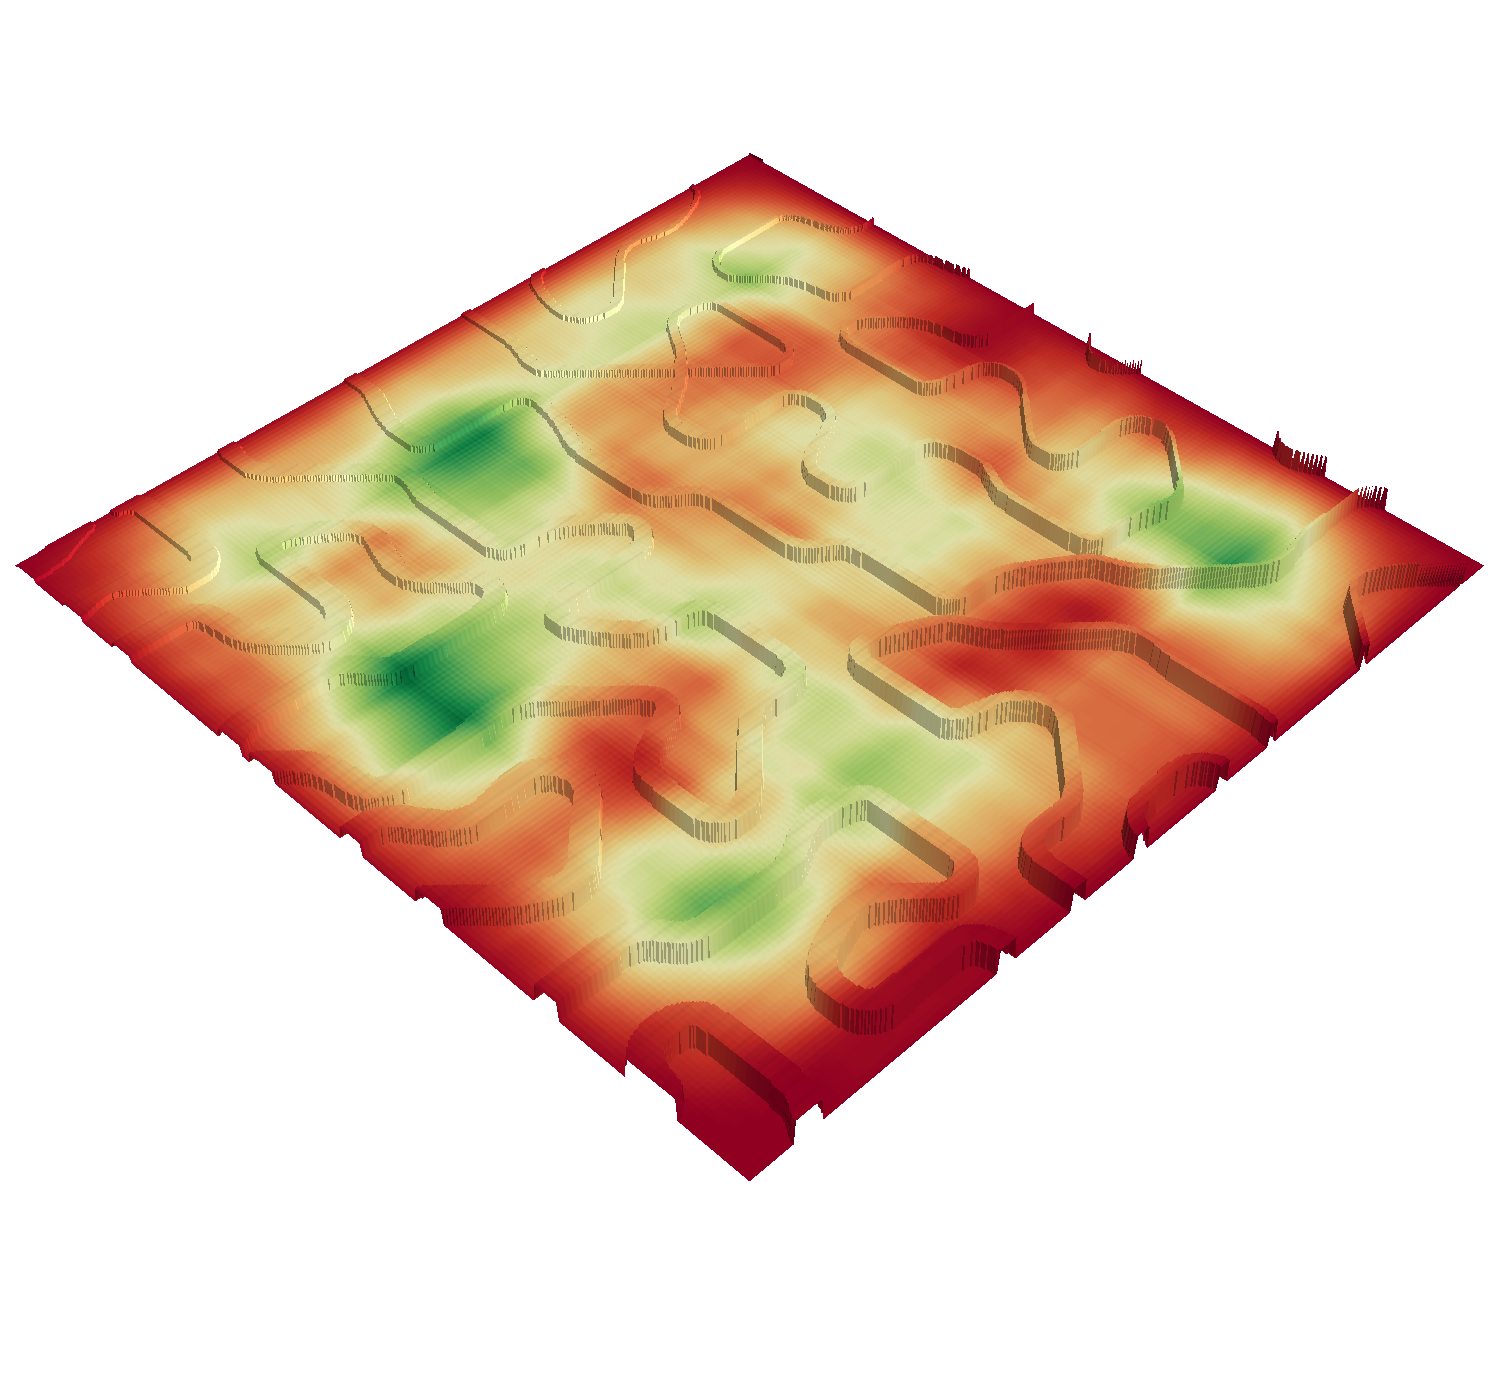
\includegraphics[width=\linewidth]{../img/4/traversability/bars/-90.png}
      \subcaption{Robot moving from top to bottom} 
      % \label{fig: bars-t2b}
  \end{subfigure}
  \begin{subfigure}[b]{0.45\textwidth}
    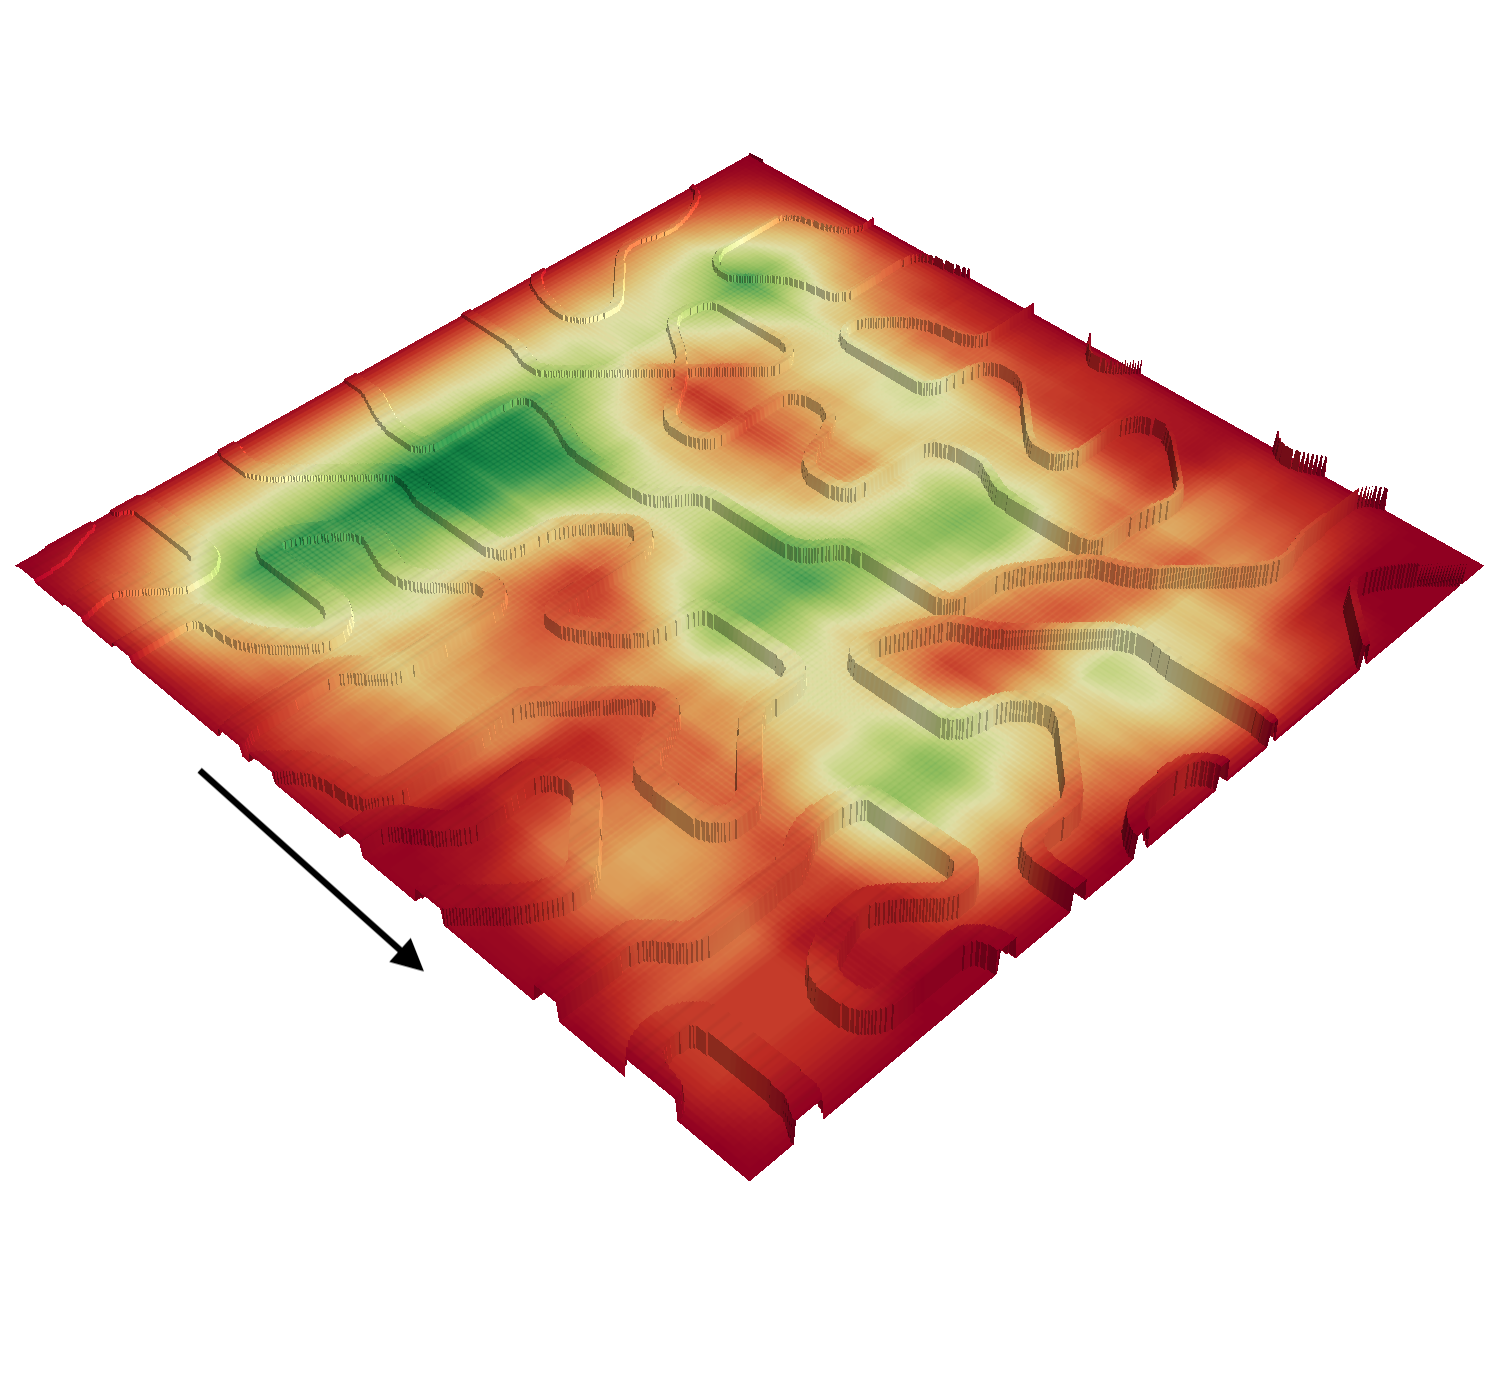
\includegraphics[width=\linewidth]{../img/4/traversability/bars/-0.png}
    \subcaption{Robot moving from left to right}   
    % \label{fig: bars-l2r}
  \end{subfigure}
  \begin{subfigure}[b]{0.45\textwidth}
      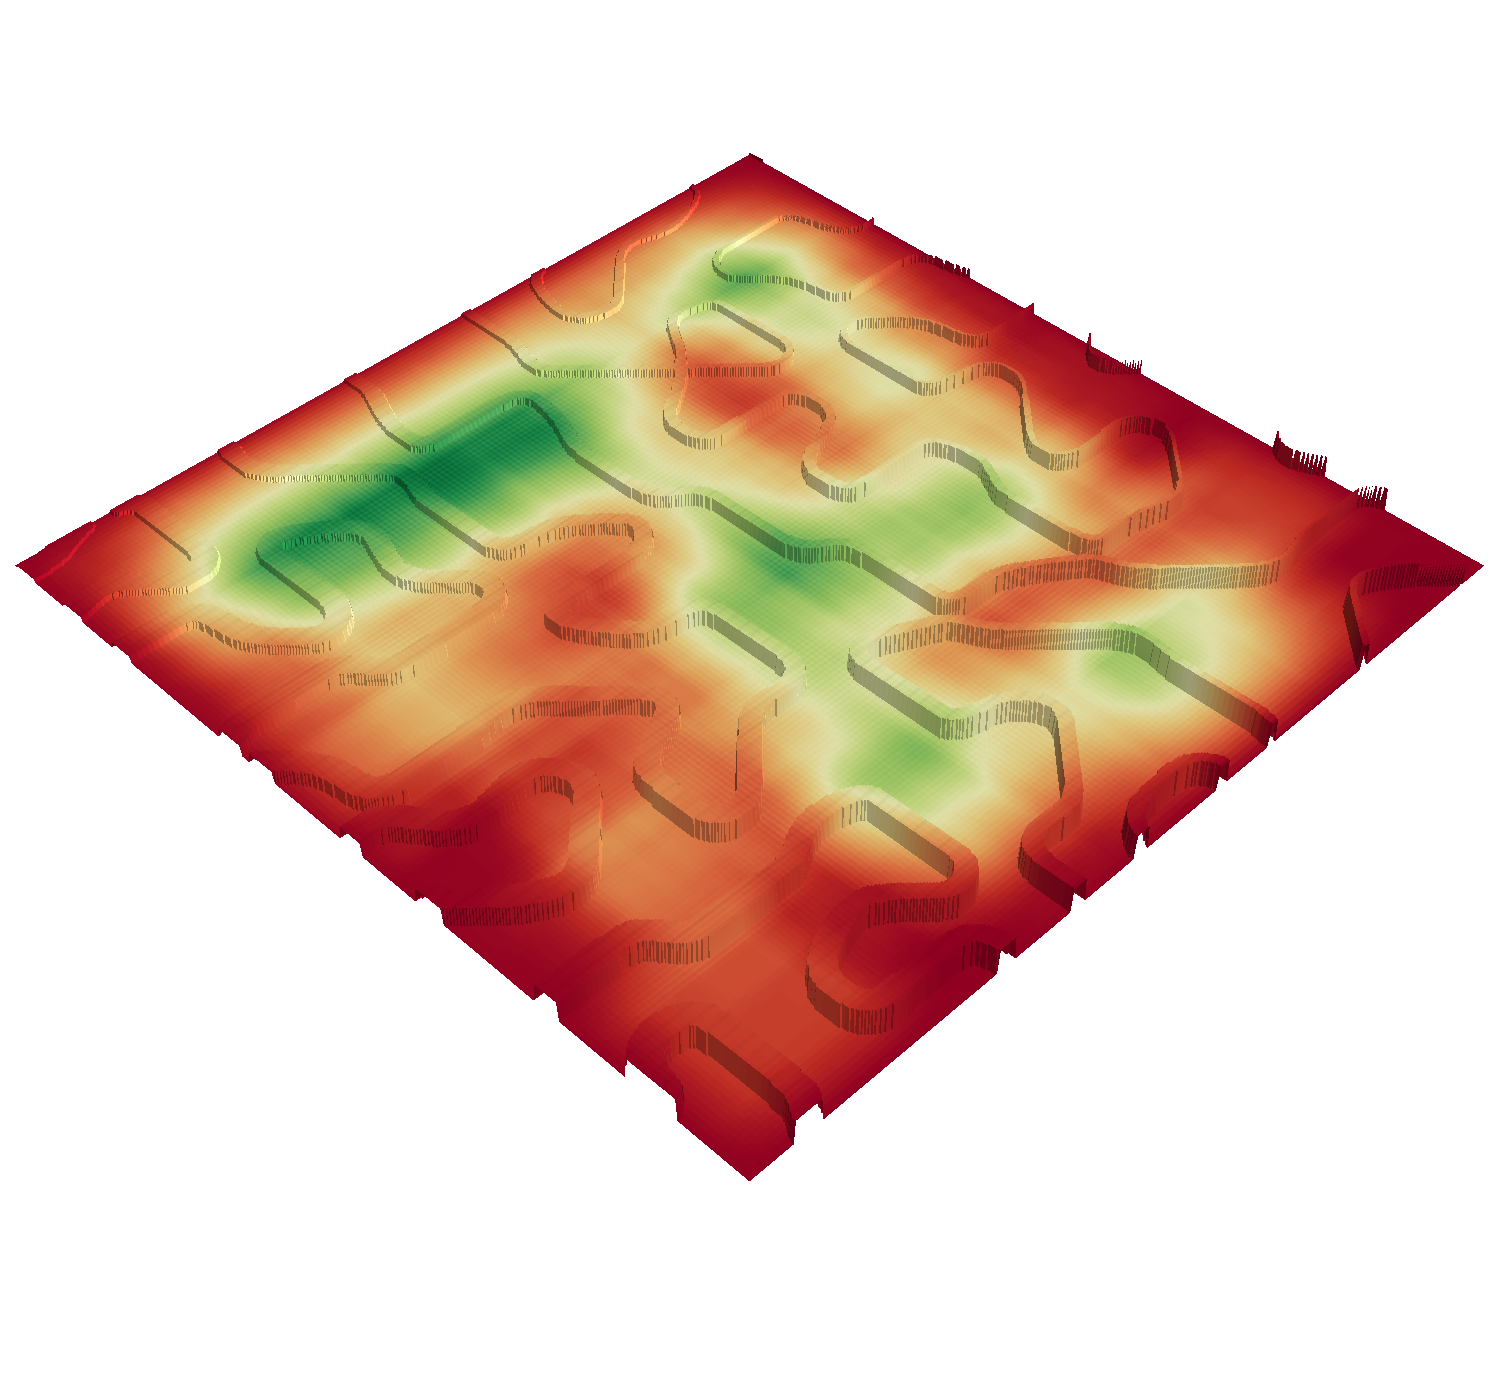
\includegraphics[width=\linewidth]{../img/4/traversability/bars/-180.png}  
      \subcaption{Robot moving from right to left} 
      % \label{fig: bars-r2l}
  \end{subfigure}
  \caption{Traversability probability on the bars map, a $10\times 10$m , for different Krock's rotation. The values are obtained by sliding a window on the map to create the patches to predict their traversability.}
  \label{fig : bars-trav}
  \end{figure}
Definitely, this was a hard map for the robot due to the high number of not traversable walls. Interesting, we can identify a tunnel near the bottom center of the maps that shows how the model correctly label those patches depending on the orientation. Figure \ref{fig : bars-tunnel-trav} highlights this detail.

\begin{figure} [htbp]
  \centering
  \begin{subfigure}[b]{0.23\textwidth}
    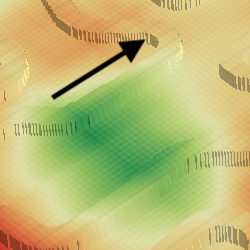
\includegraphics[width=\linewidth]{../img/4/traversability/bars/tunnel/-270-crop.png} 
    % \subcaption{Robot moving from bottom to top} 
    % \label{fig: bars-b2t}
  \end{subfigure}
  \begin{subfigure}[b]{0.23\textwidth}
      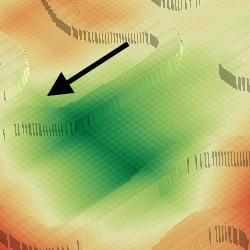
\includegraphics[width=\linewidth]{../img/4/traversability/bars/tunnel/-90-crop.png}
      % \subcaption{Robot moving from top to bottom} 
      % \label{fig: bars-t2b}
  \end{subfigure}
  \begin{subfigure}[b]{0.23\textwidth}
    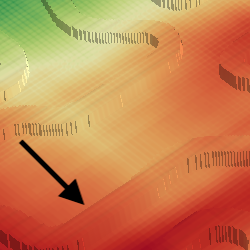
\includegraphics[width=\linewidth]{../img/4/traversability/bars/tunnel/-0-crop.png}
    % \subcaption{Robot moving from left to right}   
    % \label{fig: bars-l2r}
  \end{subfigure}
  \begin{subfigure}[b]{0.23\textwidth}
      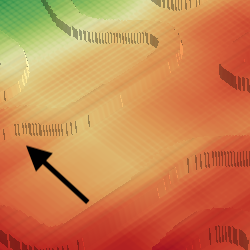
\includegraphics[width=\linewidth]{../img/4/traversability/bars/tunnel/-180-crop.png}  
      % \subcaption{Robot moving from right to left} 
      % \label{fig: bars-r2l}
  \end{subfigure}
  \caption{Detail of a region in the bars map where there are two walls forming a tunnel. Correctly, when the robot is travel following the trail the region is label as traversable.}
  \label{fig : bars-tunnel-trav}
  \end{figure}

\subsection{Small village}
We applied the same procedure to also a $10\times10$m small village map. Figure \ref{fig : small-village-trav} describes its traversability for four different rotations.

\begin{figure} [htbp]
  \centering
  \begin{subfigure}[b]{0.45\textwidth}
    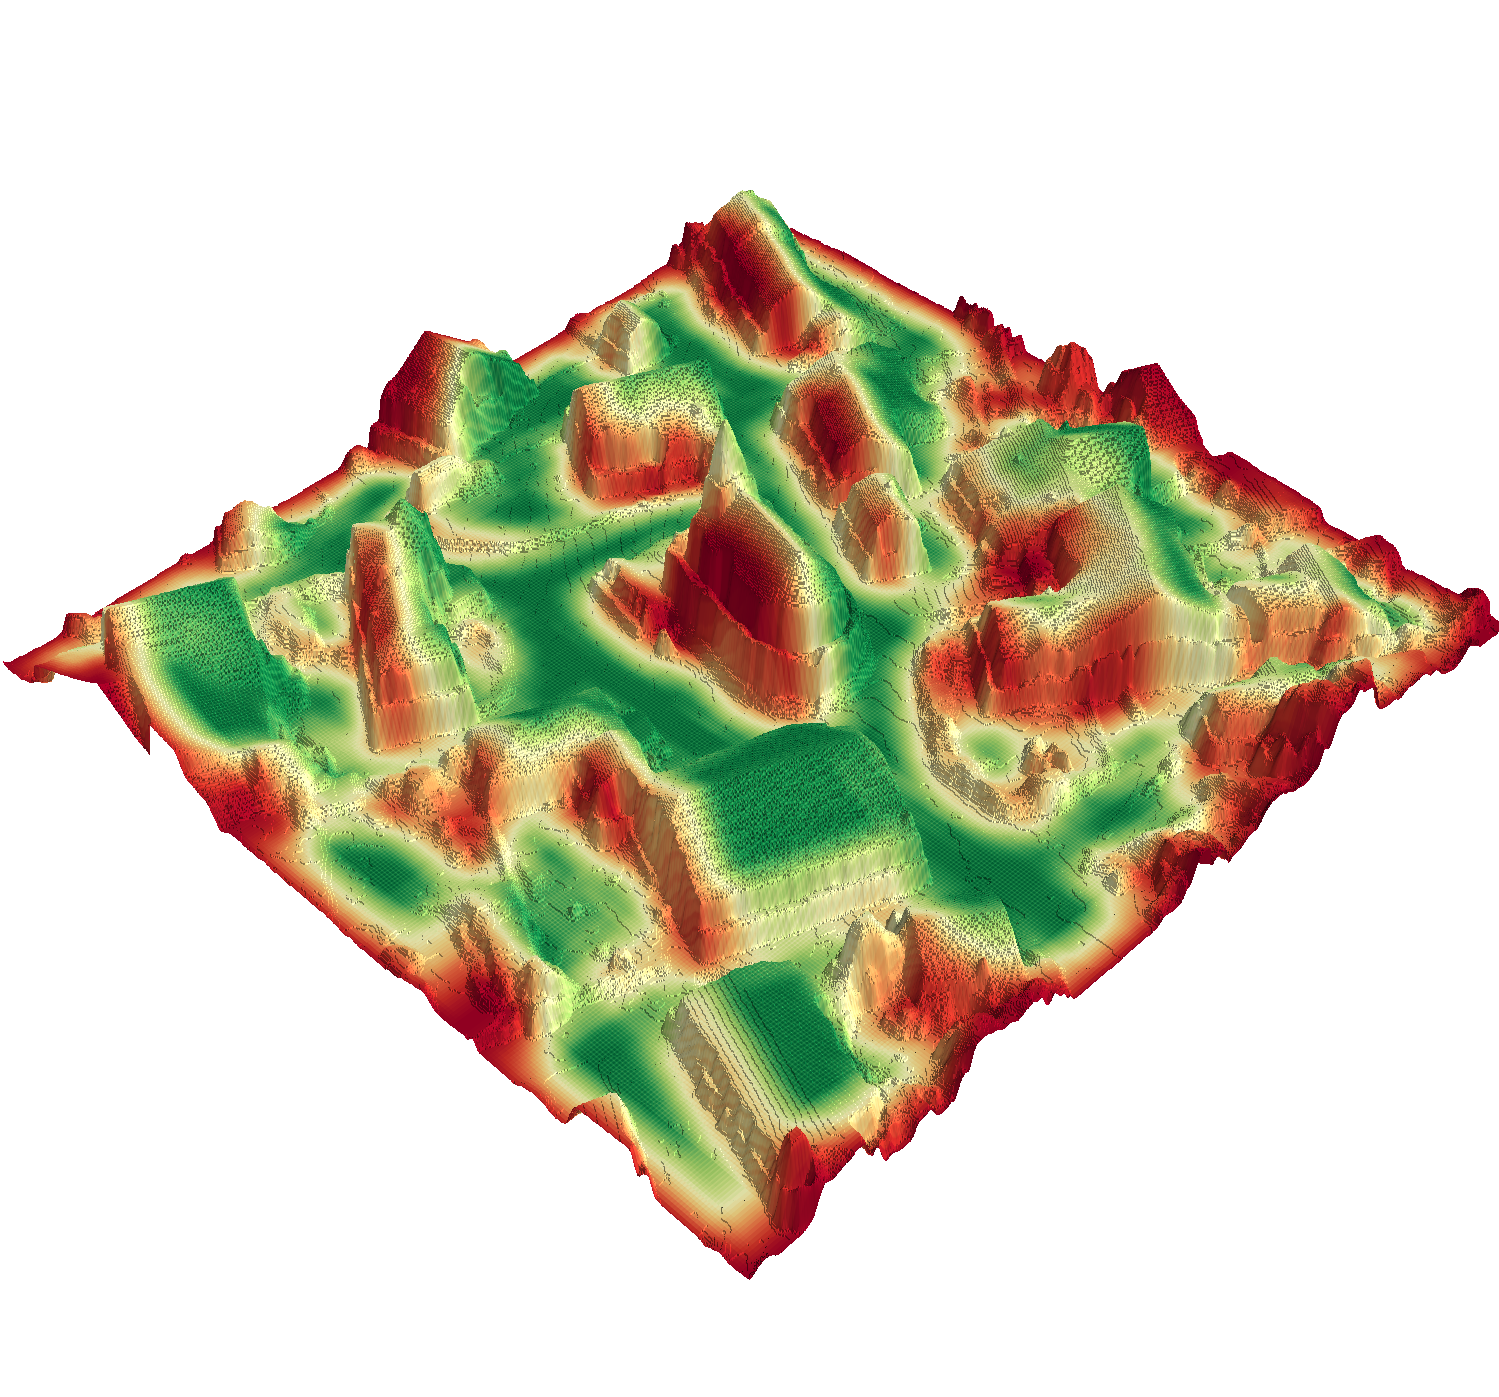
\includegraphics[width=\linewidth]{../img/4/traversability/sullens/-270.png} 
    \subcaption{Robot moving from bottom to top} 
    % \label{fig: sullens-b2t}
  \end{subfigure}
  \begin{subfigure}[b]{0.45\textwidth}
      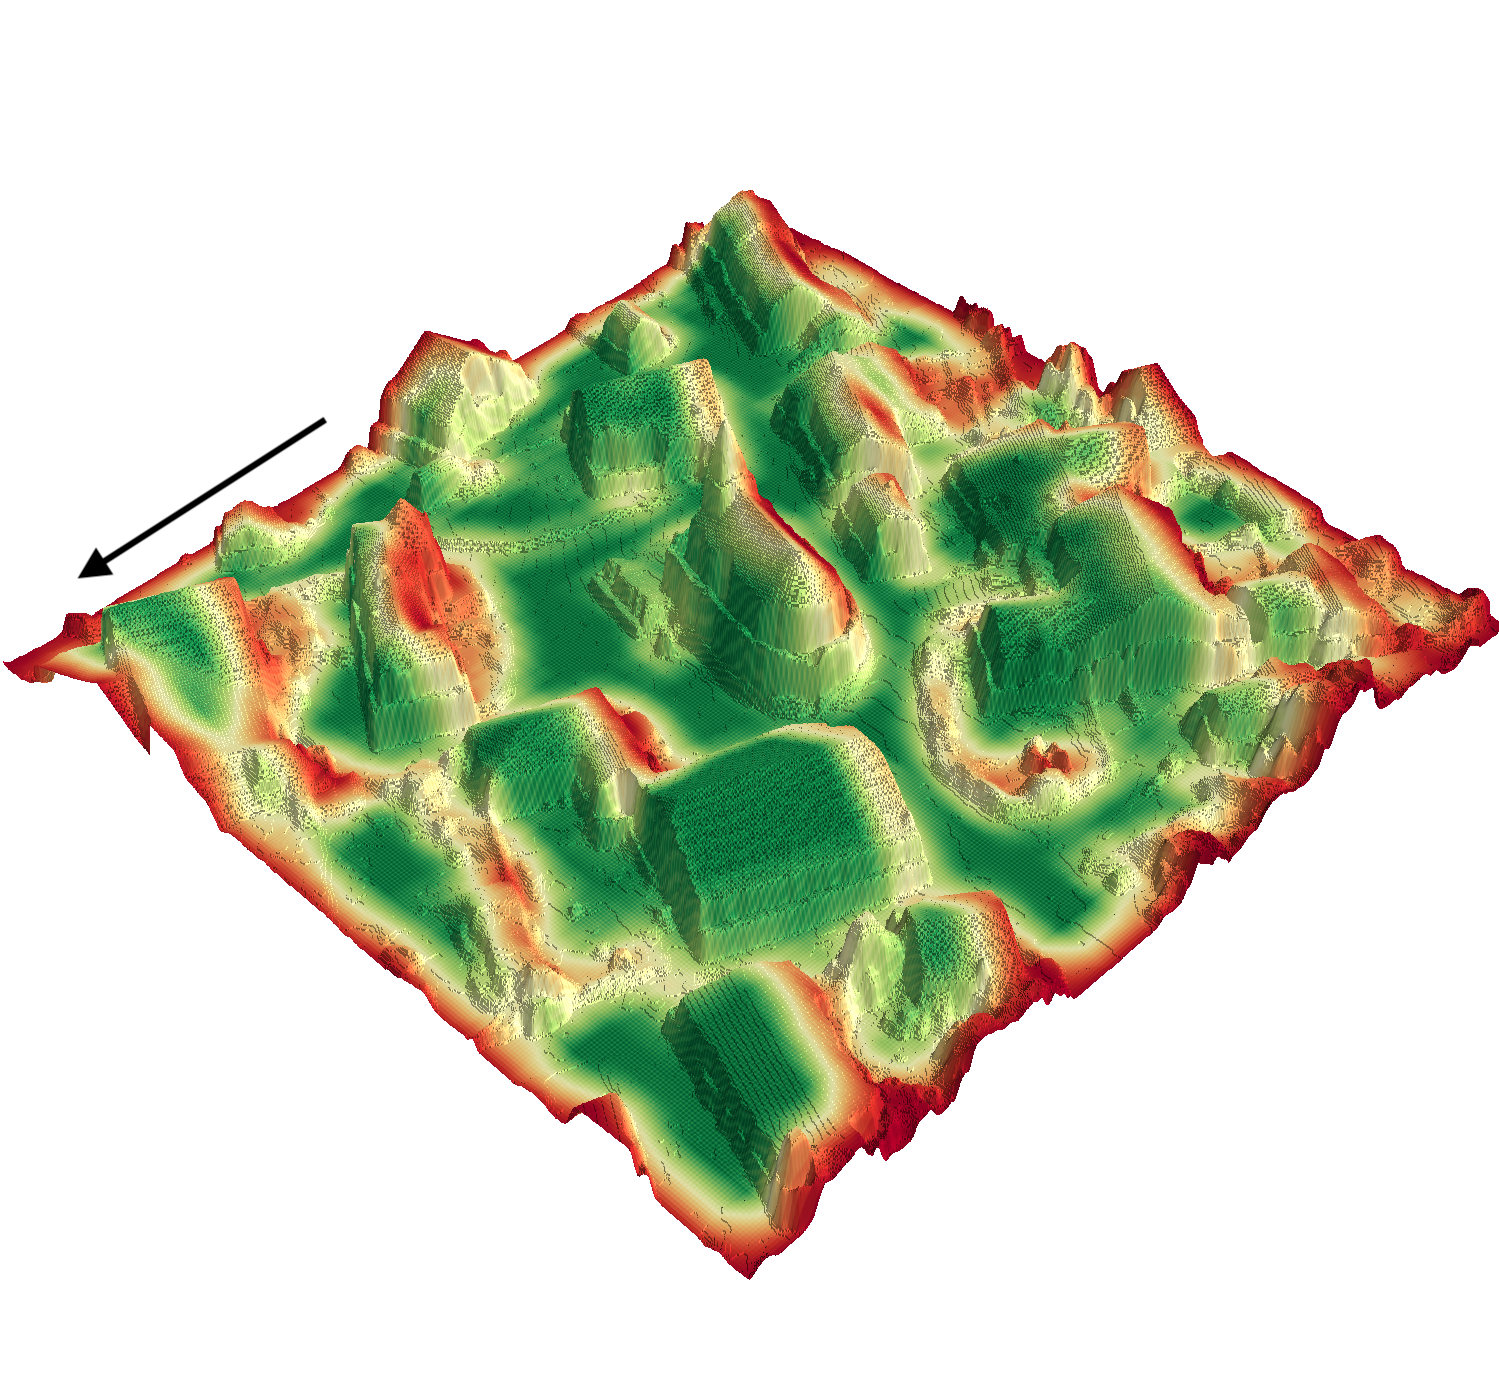
\includegraphics[width=\linewidth]{../img/4/traversability/sullens/-90.png}
      \subcaption{Robot moving from top to bottom} 
      % \label{fig: sullens-t2b}
  \end{subfigure}
  \begin{subfigure}[b]{0.45\textwidth}
    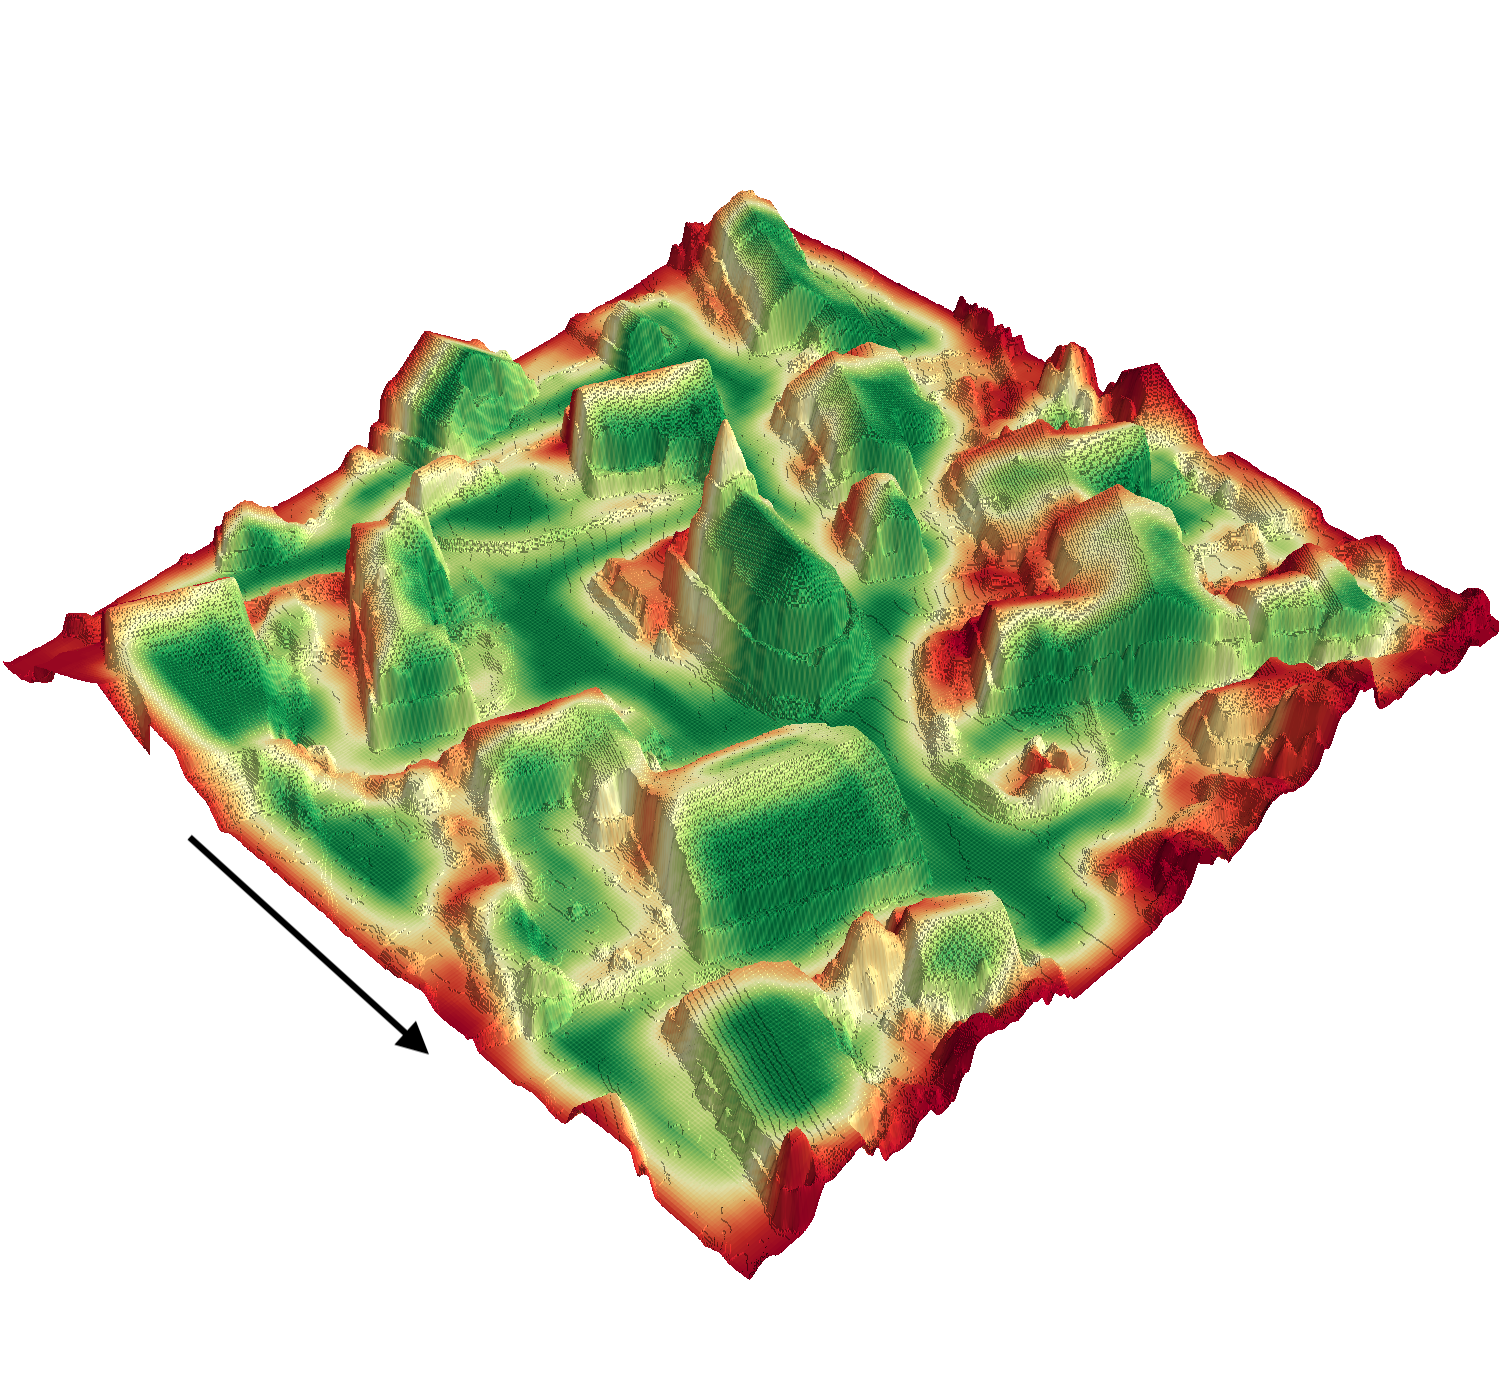
\includegraphics[width=\linewidth]{../img/4/traversability/sullens/-0.png}
    \subcaption{Robot moving from left to right}   
    % \label{fig: sullens-l2r}
  \end{subfigure}
  \begin{subfigure}[b]{0.45\textwidth}
      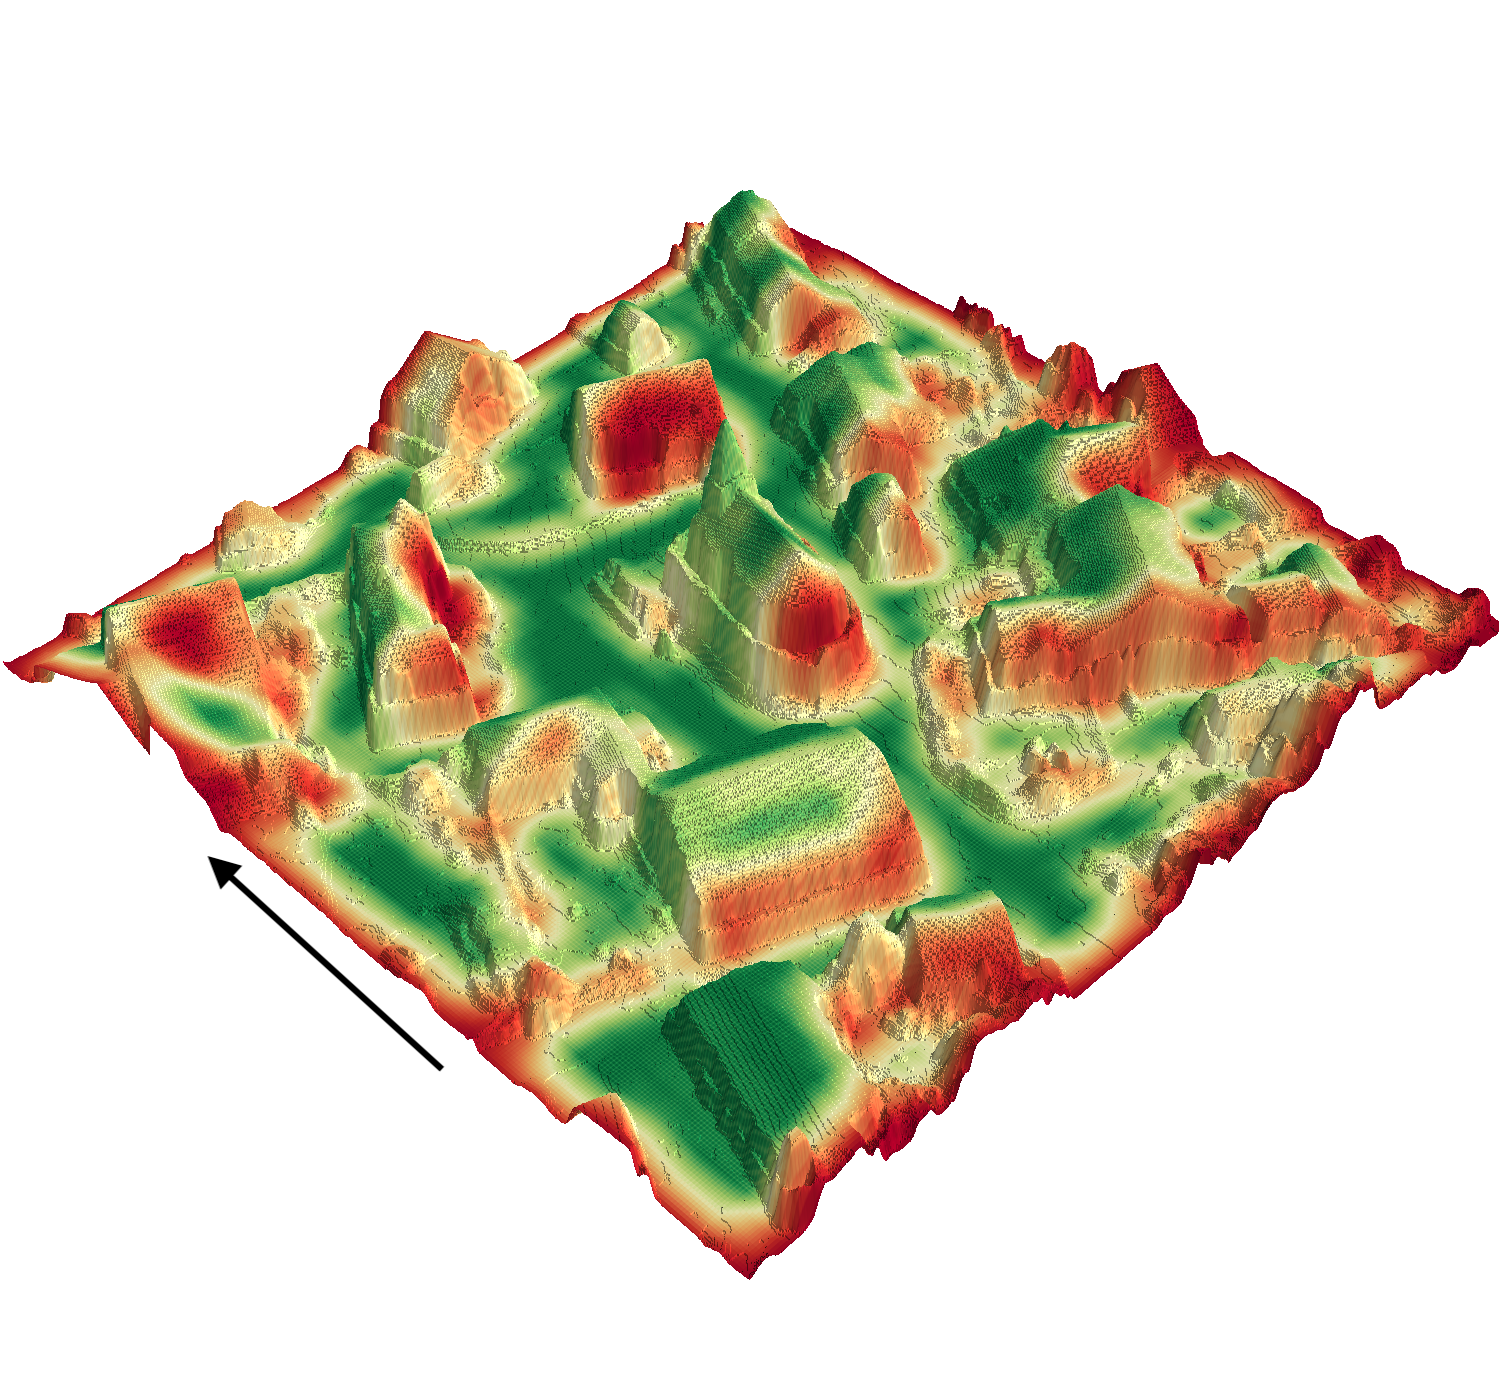
\includegraphics[width=\linewidth]{../img/4/traversability/sullens/-180.png}  
      \subcaption{Robot moving from right to left} 
      % \label{fig: bars-r2l}
  \end{subfigure}
  \caption{Traversability probability on the map of a small village for different Krock's rotation. The surface covers $30\times 30$m and has a maximum height of $10$m. The values are obtained by sliding a window on the map to create the patches to predict their traversability.}
  \label{fig : small-village-trav}
  \end{figure}
  All the streets were label as traversable, while the church's roof traversability depend on the orientation. For example, most steep roofs are not traversable when walking uphill. On the other hand, if krock walks side by side they can be traversed. Figure \ref{fig : small-village-roof-trav} shows this behavior on the church's roof.
  \begin{figure} [htbp]
    \centering
    \begin{subfigure}[b]{0.45\textwidth}
      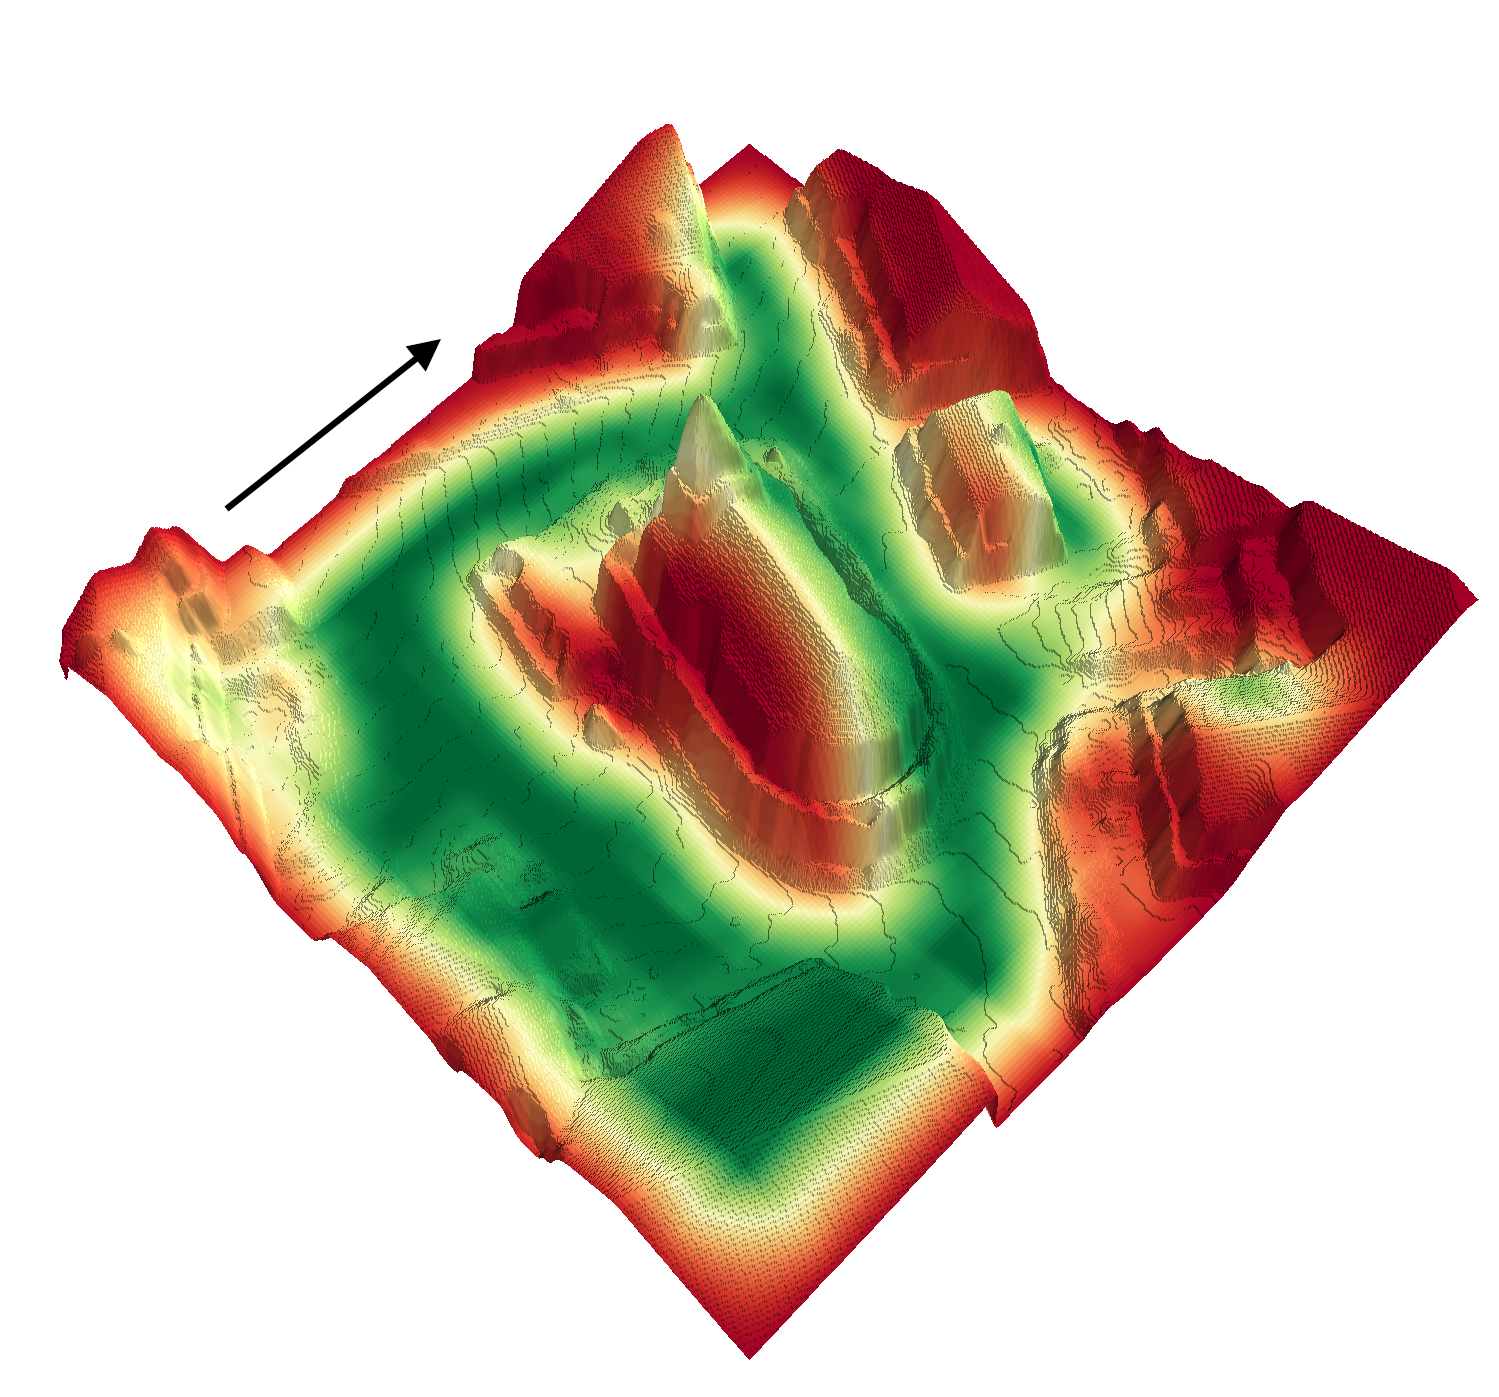
\includegraphics[width=\linewidth]{../img/4/traversability/sullens-church/-270.png} 
      \subcaption{Robot moving from bottom to top} 
      % \label{fig: sullens-b2t}
    \end{subfigure}
    \begin{subfigure}[b]{0.45\textwidth}
        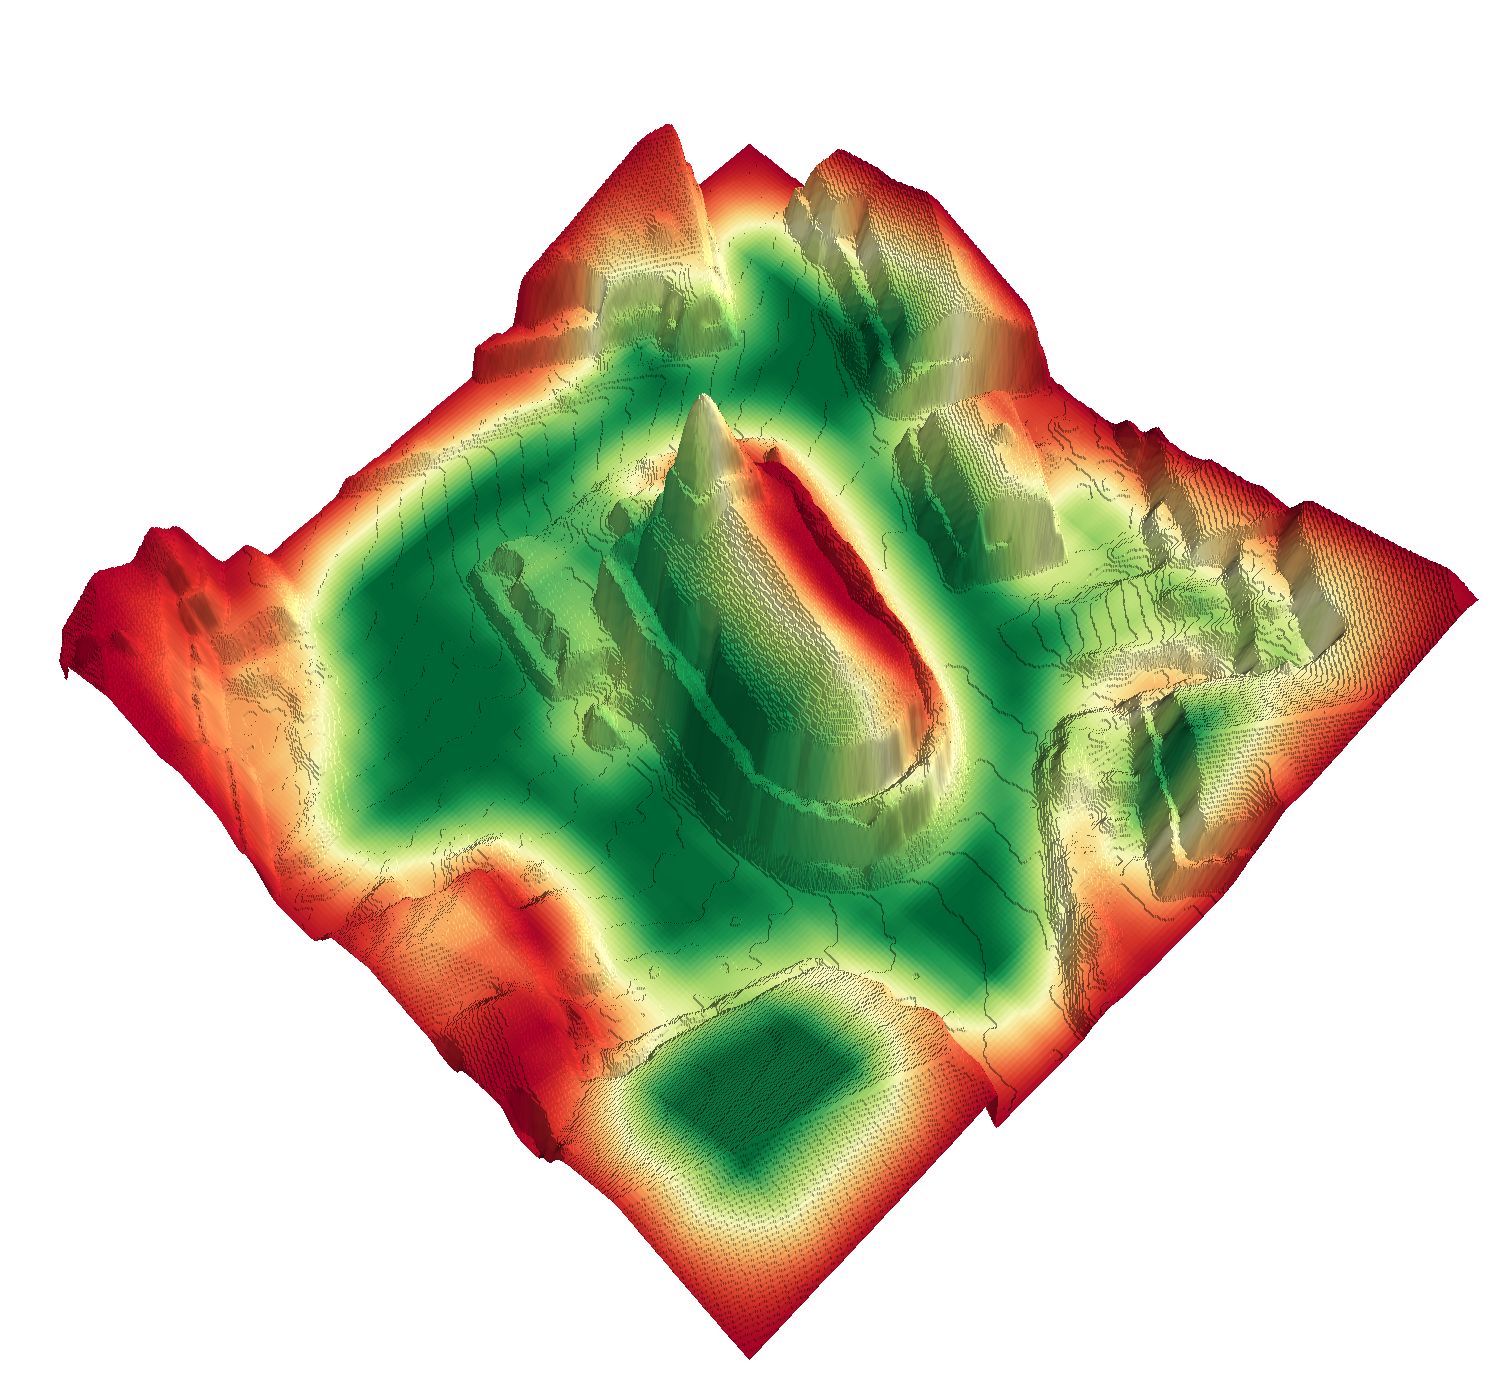
\includegraphics[width=\linewidth]{../img/4/traversability/sullens-church/-90.png}
        \subcaption{Robot moving from top to bottom} 
        % \label{fig: sullens-church-t2b}
    \end{subfigure}
    \begin{subfigure}[b]{0.45\textwidth}
      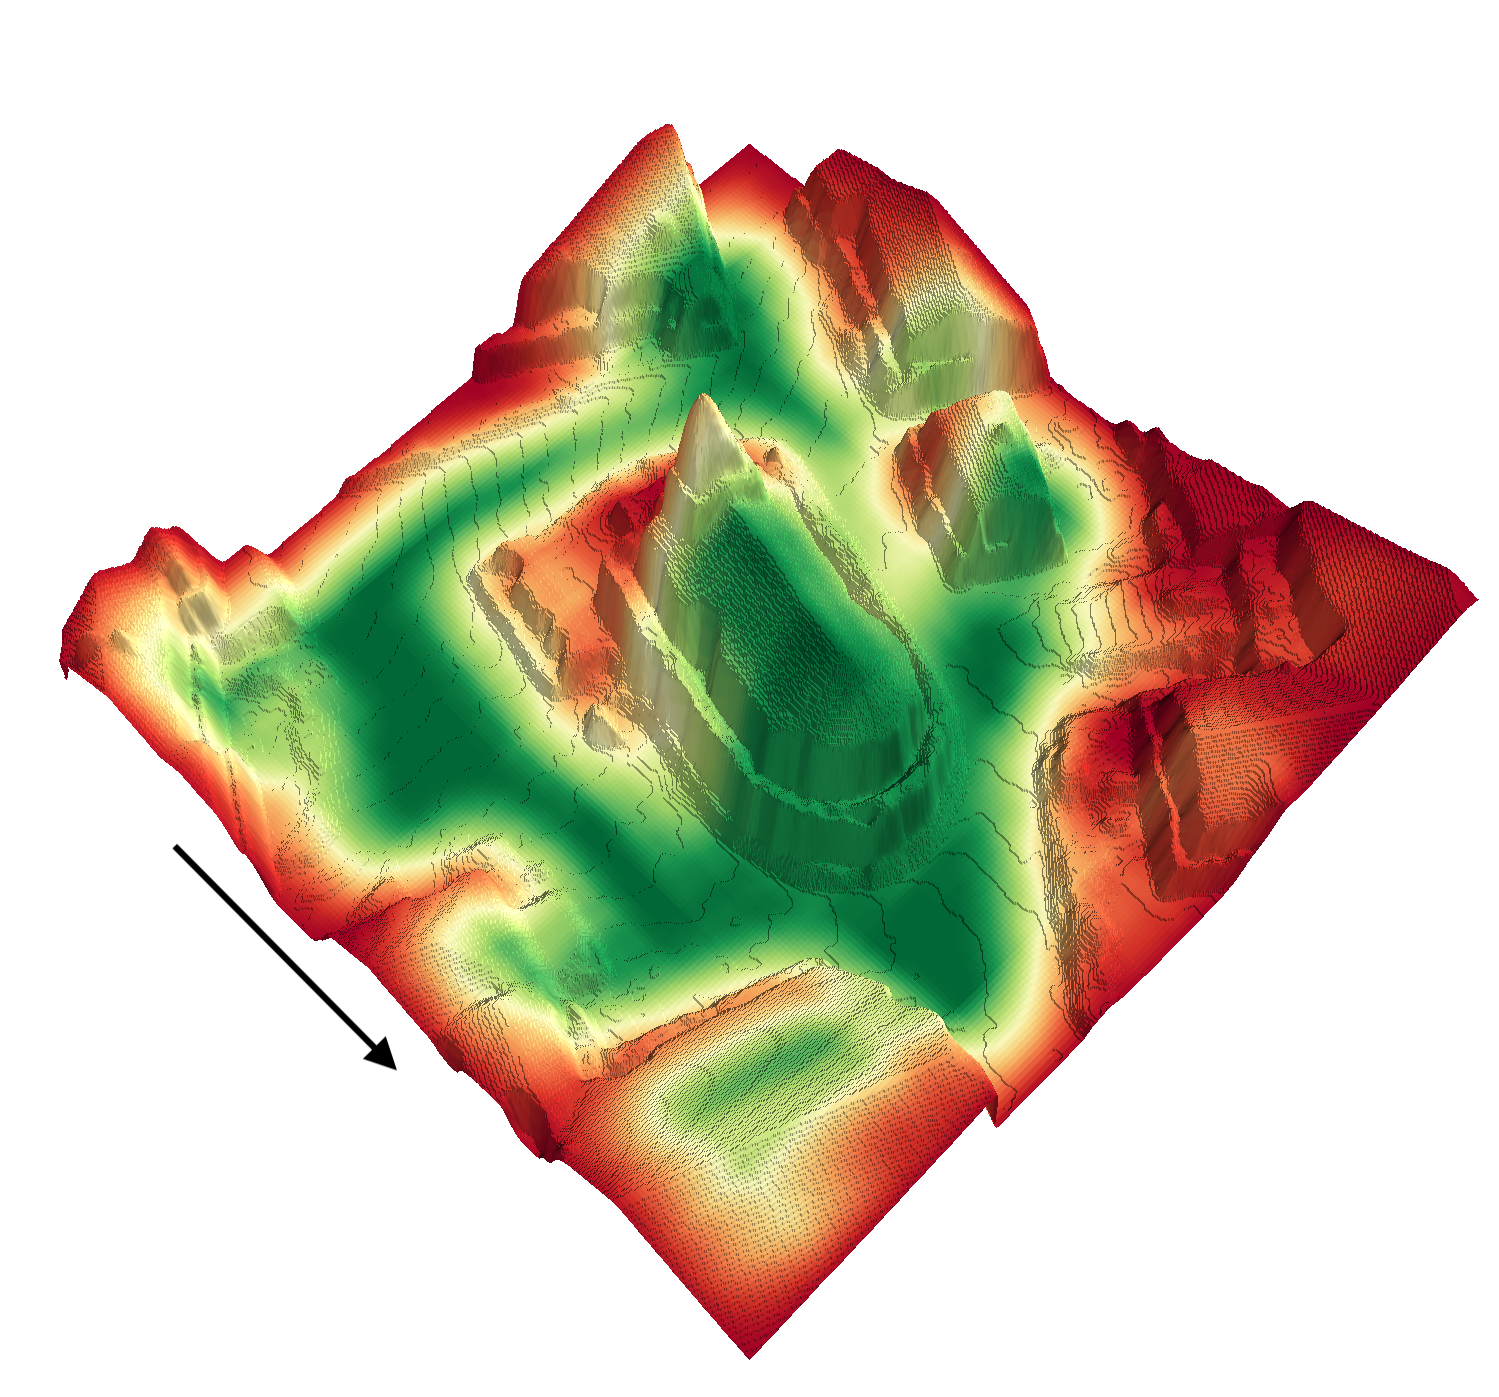
\includegraphics[width=\linewidth]{../img/4/traversability/sullens-church/-0.png}
      \subcaption{Robot moving from left to right}   
      % \label{fig: sullens-church-l2r}
    \end{subfigure}
    \begin{subfigure}[b]{0.45\textwidth}
        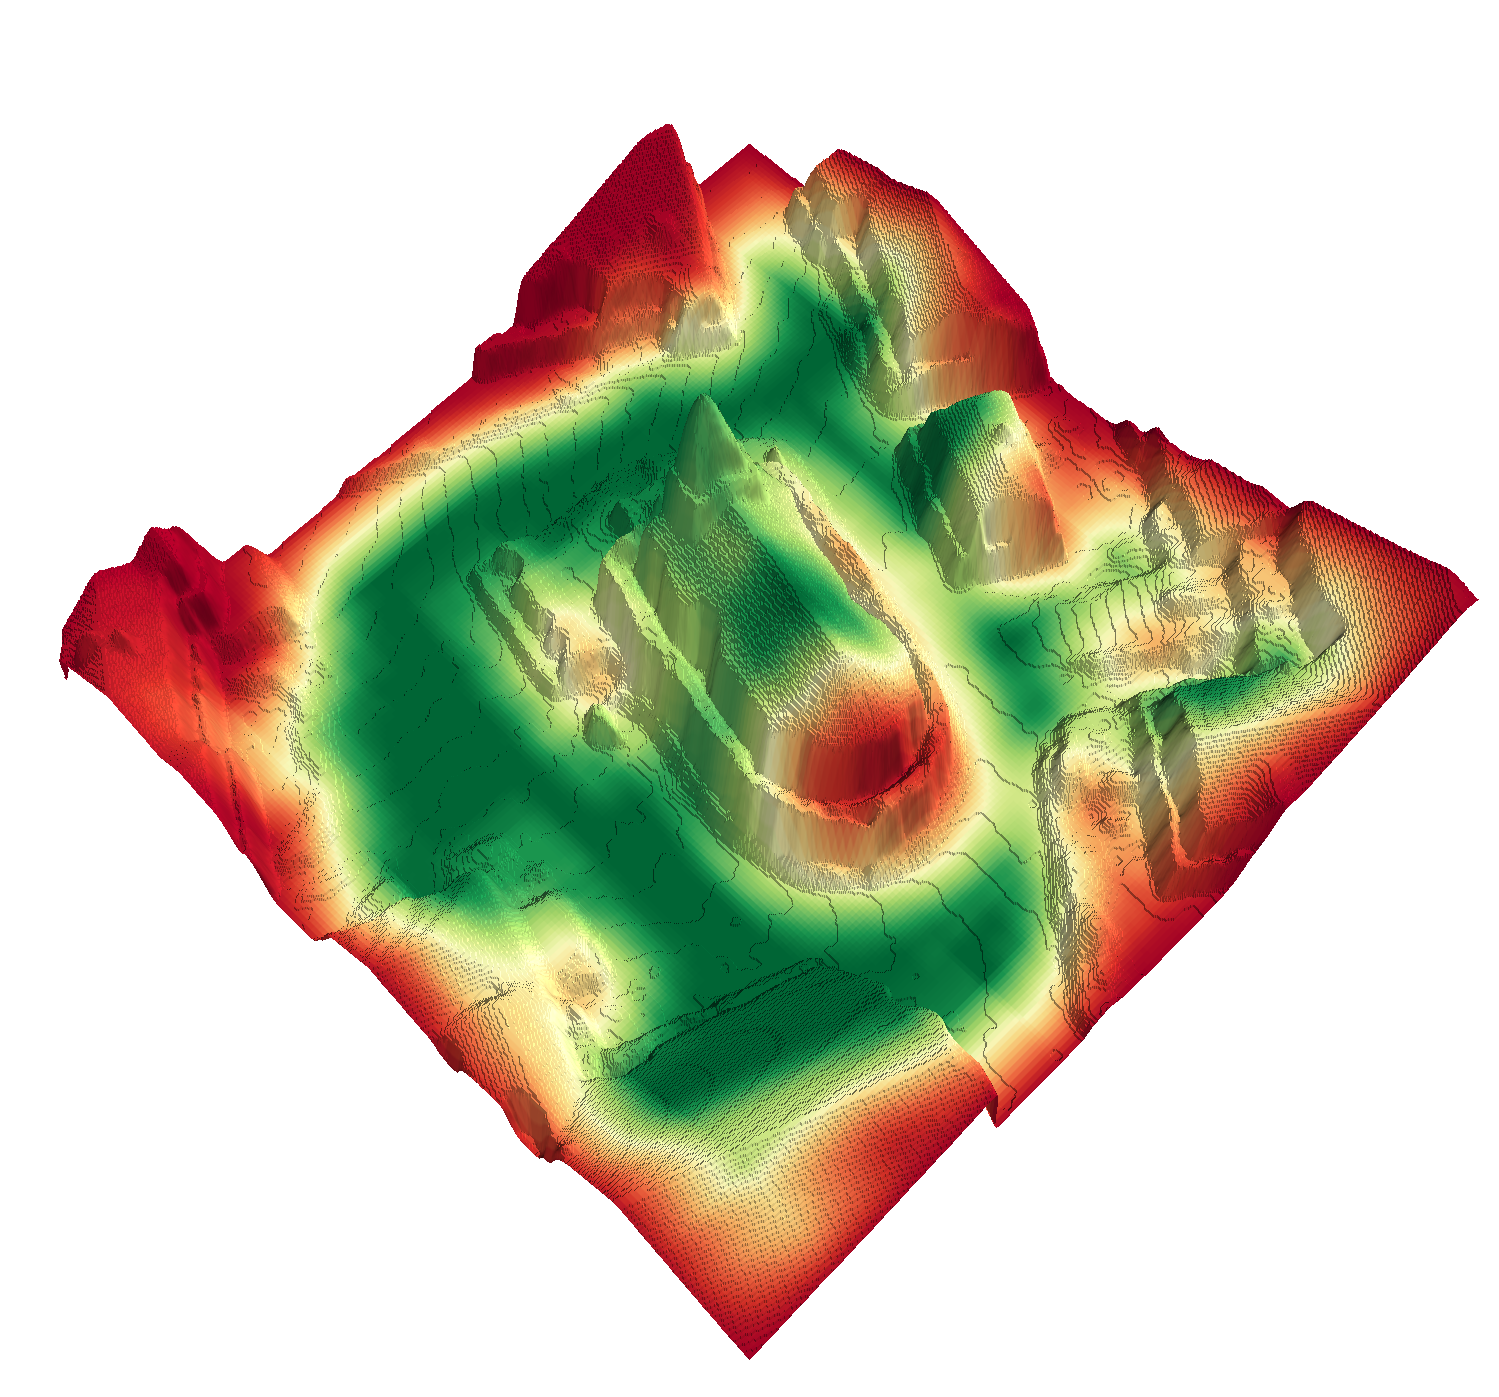
\includegraphics[width=\linewidth]{../img/4/traversability/sullens-church/-180.png}  
        \subcaption{Robot moving from right to left} 
        % \label{fig: bars-r2l}
    \end{subfigure}
    \caption{Detail of the church in the small village map for different Krock's rotation. All the fours images are correctly labeled accordingly to the robot orientation. In the first two images only downhill part of the roof is traversable. While in the last two the robot is able to travel till the end.}
    \label{fig :  small-village-roof-trav}
    \end{figure}
\end{document}